\chapter{XUV Light Source Design and Apparatus Performance}
\label{chap:XUV_source_design_performance}

\section{Introduction}

Compared to RABBITT measurements, condensed matter transient absorption experiments require a very high \textit{extreme ultraviolet} (XUV) photon flux. First, the sample thickness is usually chosen such that the XUV transmission is roughly 50\% near the spectral feature of interest. This optical density represents a compromise between the incompatible goals of having a strong ground state absorption (enabling the detection of small changes in the optical density) while simultaneously avoiding the noise floor of the detector (which is required for good statistics). Second, a high XUV flux will reduce the number of laser shots required for a given data point, which in turn reduces the total mid-infrared (MIR) flux on the sample and minimizes the effects of long-lived excited states on the measurement. Finally, a high flux reduces the overall time required to complete an experiment. This increases data fidelity by reducing the effects of unavoidable experimental noise sources such as long-term laser drift (either pointing or energy) and environmental changes caused by the building's HVAC system.

This chapter will detail the development of bright XUV sources which were required for \textit{attosecond transient absorption spectroscopy} (ATAS) experiments. It will also quantify the performance of the available XUV sources and the \textit{transient absorption beamline} (TABLe) as a whole.

\section{High Harmonic Generation (HHG) Gas Sources}
\label{sec:HHG_gas_sources}

This section will discuss the HHG gas sources used to generate harmonics for ATAS experiments. For each gas source, we will describe the device, model the gas flow and discuss their XUV output in the context of the physical principles discussed in \cref{sec:HHG}.

\subsection{Introduction}

Recalling the arguments of \cref{sec:phase-matching}, there exists an optimal phase matching pressure $P_{\textrm{opt}}$ for which the XUV flux is maximized. According to \cref{eqn:phase_matching_density}, $P_{\textrm{opt}}$ is proportional to the square of the fundamental wavelength. From \cref{eqn:HHG_Nout_2}, we expect the harmonic yield of a perfectly phase matched HHG process to scale as the square of the pressure-length product, $(PL)^2$. Additionally, we expect the harmonic yield to scale with the fundamental wavelength as $\lambda^{-(5-6)}$, as explained in \cref{sec:single-atom-response}. These factors indicate that a high interaction pressure is critical for a successful ATAS experiment.

Experimentally, the interaction pressure is a consequence of the gas flow dynamics and the design of the gas delivery device. The interaction pressure can be increased by increasing the backing pressure into the device, but this is limited by the finite pumping speed of the vacuum system. Significant improvements to both the interaction pressure $P$ and the interaction length $L$ can be made by modifying the design of the gas delivery device. The simplest and most common gas delivery device (a free expansion nozzle) cannot reach the \textit{optimum phase matching pressure} $P_{\textrm{opt}}$ at $\lambda_1 = 800 \ \textrm{nm}$ before the vacuum system is overwhelmed. Since most of our experiments are performed at longer wavelengths using the signal output of the TOPAS, and because ATAS experiments require a high XUV flux, more advanced gas delivery systems were required.

Providing the lab with a brighter harmonic source was the ultimate goal of the high pressure cell, and for the most part this goal was achieved. Below, we will review the basic design considerations, drawbacks and advantages of the four main types of gas sources used in this thesis: the free expansion nozzle, the \textit{low pressure cell} (LPC), the \textit{high pressure cell} (HPC) and the Amsterdam pulsed piezovalve. A primer on how to install and use the high pressure cell can be found in \cref{app:HPC_instructions}.

\subsection{Free Expansion Nozzle}
\label{sec:free-expansion-nozzle}

We use an \textit{in vacuo} gas nozzle to deliver a localized plume of gas near the \textit{mid-infrared} (MIR) focus. Generally, when gas flows from a high pressure region ($P_0$) to a low pressure region ($P_b$) through a small aperture of diameter $d$, a supersonic plume may form in the low pressure region. If the pressure ratio $P_0/P_b$ exceeds a critical value $G$, given by
\begin{equation}
G \equiv ((\gamma+1)/2)^{\gamma/(\gamma-1)} \le 2.1,
\label{eqn:G_factor}
\end{equation}
then the gas flow at the aperture will be equal to the speed of sound, and the pressure will be equal to $P_0 / G \approx P_0/2$. The highest chamber pressures in our experiments are on the order of $P_b \approx 10$ mTorr, and typical backing pressures for harmonic generation generally exceed 50 Torr, so we are always operating with a supersonic jet. The on-axis spatial extent of the supersonic gas plume is estimated by the Mach disk location, $x_M$:
\begin{equation}
x_M / d = 0.67 \sqrt{P_0/P_b}.
\label{eqn:Mach-disk}
\end{equation}
For a chamber pressure of 3 mTorr and a backing pressure of 450 Torr, ${x_M = 260d = 51.9 \ \textrm{mm}}$ for a 200 $\mu$m diameter aperture. As will be shown below, our laser-gas interaction region is well within the structure of the gas jet.

\begin{table}[]
	\centering
	\begin{tabular}{lllllllll}
		\hline
		\multicolumn{1}{c}{Source} & \multicolumn{1}{c}{$j$} & \multicolumn{1}{c}{$\gamma$} & \multicolumn{1}{c}{$C_1$} & \multicolumn{1}{c}{$C_2$} & \multicolumn{1}{c}{$C_3$} & \multicolumn{1}{c}{$C_4$} & \multicolumn{1}{c}{$A$} & \multicolumn{1}{c}{$B$} \\ \hline
		3D                         & 1                     & 5/3                          & 3.232                     & -0.7563                   & 0.3937                    & -0.0729                   & 3.337                & -1.541                \\
		3D                         & 1                     & 7/5                          & 3.606                     & -1.742                    & 0.9226                    & -0.2069                   & 3.190                 & -1.610                \\
		3D                         & 1                     & 9/7                          & 3.971                     & -2.327                    & 1.326                     & -0.311                    & 3.609                 & -1.950                \\
		2D                         & 2                     & 5/3                          & 3.038                     & -1.629                    & 0.9587                    & -0.2229                   & 2.339                 & -1.194                \\
		2D                         & 2                     & 7/5                          & 3.185                     & -2.195                    & 1.391                     & -0.3436                   & 2.261                 & -1.224                \\
		2D                         & 2                     & 9/7                          & 3.252                     & -2.473                    & 1.616                     & -0.4068                   & 2.219                 & -1.231               
	\end{tabular}
	\caption{Gas parameters used in \cref{eqn:Scoles_centerline2.2}. Table recreated from Ref \cite{millerFreeJetSources1988}.}
	\label{tbl:Scoles_gas_params2.2}
\end{table}

The physics of supersonic gas flow have been discussed at length in the literature, so we will only go over the relevant highlights \cite{millerFreeJetSources1988,joustenHandbookVacuumTechnology2016}. The ratio of the velocity of the gas $V$ to the speed of sound $a$ is called the \textit{Mach number} $M=V/a$. It can be shown that all thermodynamic parameters within the supersonic structure (density, pressure, velocity and temperature) can be expressed in terms of the Mach number and the heat capacity ratio $\gamma$. For harmonic generation, we are primarily concerned with the on-axis ($y=0$) mass density $\rho$ and pressure $P$:
\begin{subequations}
	\label{eqn:mach_properties}
	\begin{align}
	\frac{\rho}{\rho_0} = \frac{n}{n_0} = \left(\frac{T}{T_0}\right)^{1/(\gamma-1)} &= \left(  1 + \frac{\gamma-1}{2} M^2 \right)^{-1/(\gamma-1)} \label{eqn:mach_rho}, \\
	\frac{P}{P_0} = \left(\frac{T}{T_0}\right)^{\gamma/(\gamma-1)} &= \left(  1 + \frac{\gamma-1}{2} M^2 \right)^{-\gamma/(\gamma-1)} \label{eqn:mach_pressure}.
	\end{align}
\end{subequations}

Here, $\rho_0$ is the mass density at the nozzle aperture ($x=0$), and $n$ is the number density. The Mach number is found by solving the fluid mechanics equations dealing with the conversation of mass, momentum and energy for a given nozzle geometry. For a complete discussion, see \cite{millerFreeJetSources1988}. Below we present the on-axis result, which is an analytic fit to a numerical solution of the thermodynamic equations:
\begin{subequations}
	\label{eqn:Scoles_centerline2.2}
	\begin{align}
	% eqns from table 2.2 of scoles, page 23
	\frac{x}{d} > 0.5&: &&M = \left( \frac{x}{d} \right)^{(\gamma-1)/j} \left[ C_1 + \frac{C_2}{\left(\frac{x}{d}\right)} + \frac{C_3}{\left(\frac{x}{d}\right)^2} + \frac{C_4}{\left(\frac{x}{d}\right)^3} \right] \label{eqn:Scoles_centerline1}, \\
	0 < \frac{x}{d} < 1.0&: &&M = 1.0 + A \left( \frac{x}{d} \right)^2 + B \left( \frac{x}{d} \right)^3. \label{eqn:Scoles_centerline2}
	\end{align}
\end{subequations}
The fitting coefficients for \cref{eqn:Scoles_centerline2.2} are listed in \cref{tbl:Scoles_gas_params2.2}. We can see that $M$ scales with powers of $x/d$, the number of nozzle diameters away from the nozzle aperture.

The gas nozzle throughput $\hat{T}$ is proportional to the area of the aperture and the backing pressure:
\begin{equation}
\hat{T} \ (\text{Torr} \cdot \text{l}/\text{s}) = c \left(\frac{T_C}{T_0} \right)\sqrt{\frac{300}{T_0}} P_0 d^2,
\label{eqn:nozzle_thruput}
\end{equation}
where $c$ is a gas constant\footnote{Values of $c$ for common gas species are listed here: 45 [He], 20 [Ne], 14 [Ar], 16 [N\textsubscript{2}] in l/cm\textsuperscript{2}/s. For a full table of values, see Table 2.5 in \cite{millerFreeJetSources1988}.}, $T_C$ and $T_0$ are the vacuum chamber and backing temperatures, respectively, and $d$ is the nozzle diameter in cm. Ignoring the effect of the generation chamber's vacuum aperture, we can estimate the operating pressure of the generation chamber $P_b$ using the following equation \cite{hablanianHighvacuumTechnologyPractical1997}:
\begin{equation}
P_b \ (\text{Torr}) = \frac{\hat{T}}{S},
\end{equation}
where $S$ is the pumping speed of the turbo pump in liters per second. To avoid overloading our turbo pumps, we are typically limited to operating pressures below 5 -- 10 mTorr.

\begin{figure}
	\centering
	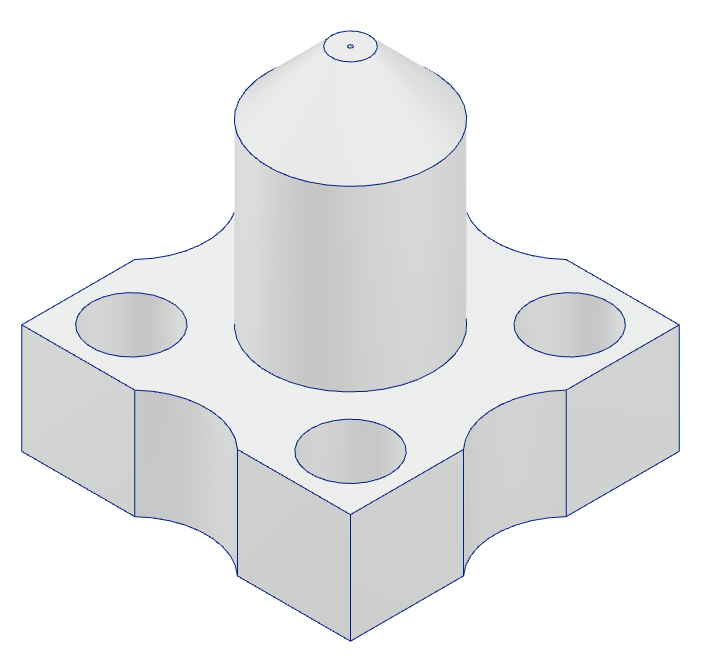
\includegraphics[width=0.5\textwidth]{figures/chap3/gas_nozzle.png}
	\caption{Rendering of the continuous free expansion nozzle. Gas flows from the base of the nozzle (bottom) and out of the 200 $\mu$m aperture (top). The top surface is beveled so the nozzle can be brought closer to the MIR focus without clipping the beam.}
	\label{fig:gas_nozzle}
\end{figure}

The basic design of our continuous free expansion nozzle is shown in \cref{fig:gas_nozzle}. The nozzle is an aluminum cylinder with a small diameter hole drilled into the top surface. Gas is delivered to the aperture via a universal gas receiver (not shown), which attaches to base of the nozzle. To reduce the gas load on the pumps, we used a $200 \ \mu m$ diameter aperture, which was the smallest size hole the machine shop could readily drill into aluminum. A 200 $\mu$m diameter aperture backed with 180 Torr of argon will deliver a gas throughput of approximately {1 Torr $\cdot$ l/s}. With a pumping speed of $S = 1000$ l/s, the generation chamber pressure will be around $P_b = 1$ mTorr. For a monatomic gas, $G = 2.05$, and the pressure at the nozzle aperture is $P_0/G \approx 87 \textrm{ Torr}$.

\begin{figure}
	\centering
	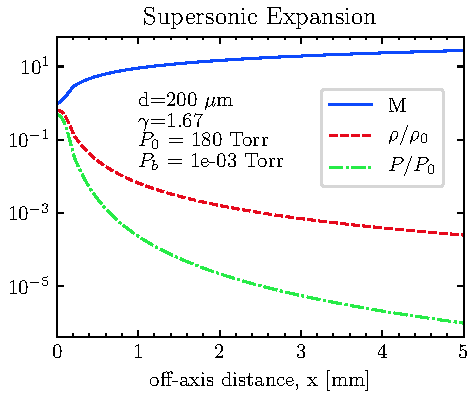
\includegraphics[width=0.75\textwidth]{figures/chap3/M_rho_P_vs_x.pdf}
	\caption{On-axis Mach number $M$, mass density $\rho$ and pressure $P$ for a free expansion nozzle.}
	\label{fig:M_rho_vs_x}
	% \Python Scripts\HPC\HPCvsLPC.py
\end{figure}


The on-axis Mach number, density and pressure for a monatomic gas are shown in \cref{fig:M_rho_vs_x}. We can see the on-axis gas density drops off precipitously with increasing distance from the nozzle aperture $x$. Recalling \cref{fig:Constant1999_fig1}, we want to bring the nozzle as close to the optical axis to maximize the interaction density. However, if nozzle face enters the focal volume it will be drilled by the high intensity light and the resulting metallic plume will coat the generation chamber's vacuum window. Under normal operating conditions, we estimate the optical axis is located at $x=100 \ \mu$m.

\begin{figure}
	\centering
	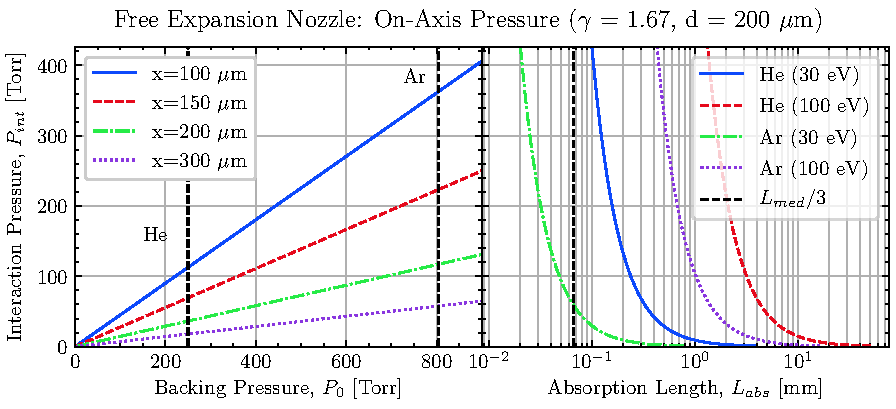
\includegraphics[width=1.0\textwidth]{figures/chap3/on-axis-pressure.pdf}
	\caption{On-axis interaction pressure and absorption length for the free expansion nozzle. Left panel: On-axis pressure as a function of nozzle backing pressure for various on-axis distances $x$. Vertical dashed lines indicate pressures at which the vacuum system is overwhelmed (5 mTorr). Right panel: Required average interaction pressure as a function of absorption length $L_{abs}$ for both gases at 30 and 100 eV.}
	\label{fig:on-axis-pressure}
	% \Python Scripts\HPC\HPCvsLPC.py
\end{figure}

The left panel of \cref{fig:on-axis-pressure} shows the on-axis interaction pressure for He and Ar ($\gamma = 5/3$) as a function of the nozzle backing pressure at various on-axis distances. Vertical dashed lines correspond to the highest sustainable backing pressure for each gas. For $x/d = 1$, the maximum interaction pressure for argon is $\sim 120$ Torr and for helium it is $\sim 35$ Torr; for $x/d = 2$, $P_{int}(Ar) \sim 360$ Torr and $P_{int}(He) \sim 110$ Torr.

Recalling the results of the 1D reabsorption model discussed in \cref{sec:XUV_reabsorption}, ideal phase matching occurs if the \textit{interaction length} ($L_{\textrm{med}}$) more than three times greater than the \textit{absorption length} ($L_{\textrm{abs}}$): $L_{\textrm{med}} > 3 L_{\textrm{abs}}$. We can estimate the absorption length of the gas plume by assuming a boxcar function density profile of width $d$. Note that this approximation overestimates the average density in the interaction region, as the off-axis density profile at large values of $x/d$ is proportional to $\cos^4 \theta$, where $\tan \theta \equiv y/x$ \cite{millerFreeJetSources1988}. Therefore $d/3$ represents a hard upper bound for $L_{\textrm{abs}}$, which is 67 $\mu$m for a 200 $\mu$m nozzle. The right panel of \cref{fig:on-axis-pressure} shows the absorption length for both gasses at 30 and 100 eV. We can see that the free expansion nozzle is only capable of phase matching argon at lower photon energies, where the XUV absorption cross section is larger. The free expansion nozzle is incapable of properly phase matching helium at any photon energy.

\subsection{Low Pressure Cell (LPC)}
\label{sec:LPC}

\begin{figure}
	\centering
	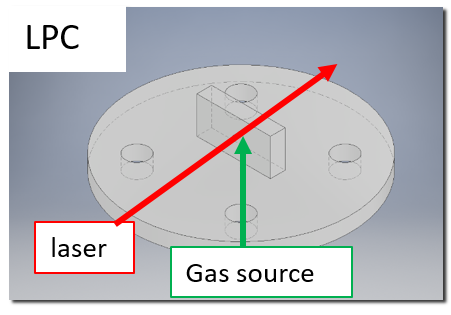
\includegraphics[width=0.5\textwidth]{figures/chap3/LPC_diagram.png}
	\caption{Rendering of the low pressure cell (LPC). The interaction region is contained within the rectangular block. The circular disk is attached to the universal gas receiver (not shown) via the four through holes.}
	\label{fig:LPC_diagram}
	% figure created in Chap 3 figures powerpoint.
\end{figure}

We have shown that the free expansion nozzle cannot provide sufficiently high pressure-length product to phase match high energy photons. The \textit{low pressure cell} (LPC), shown in \cref{fig:LPC_diagram}, was designed to improve the ratio $L_{\textrm{abs}} / L_{\textrm{med}}$ while maintaining a relatively simple nozzle geometry \cite{wangMidinfraredStrongfieldLaser2018}.\footnote{Special thanks to Zhou Wang for designing the original LPC. The LPC used in this work has been slightly modified to work with our universal gas receiver.} The LPC consists of an aluminum disk with rectangular block at the center of the top surface. Gas flows from the universal gas receiver (which is mated to the bottom of the disk) through a thin capillary and into the rectangular block. A through hole drilled into the front face of the rectangular block intersects the capillary and serves as the gas-laser interaction volume. Below, we will model the gas density profile of the LPC and show that the thickness of the block ($W = 2.032$ mm) sets the gas-laser interaction length.

\subsubsection{Gas Flow in the LPC}

\begin{figure}
	\centering
	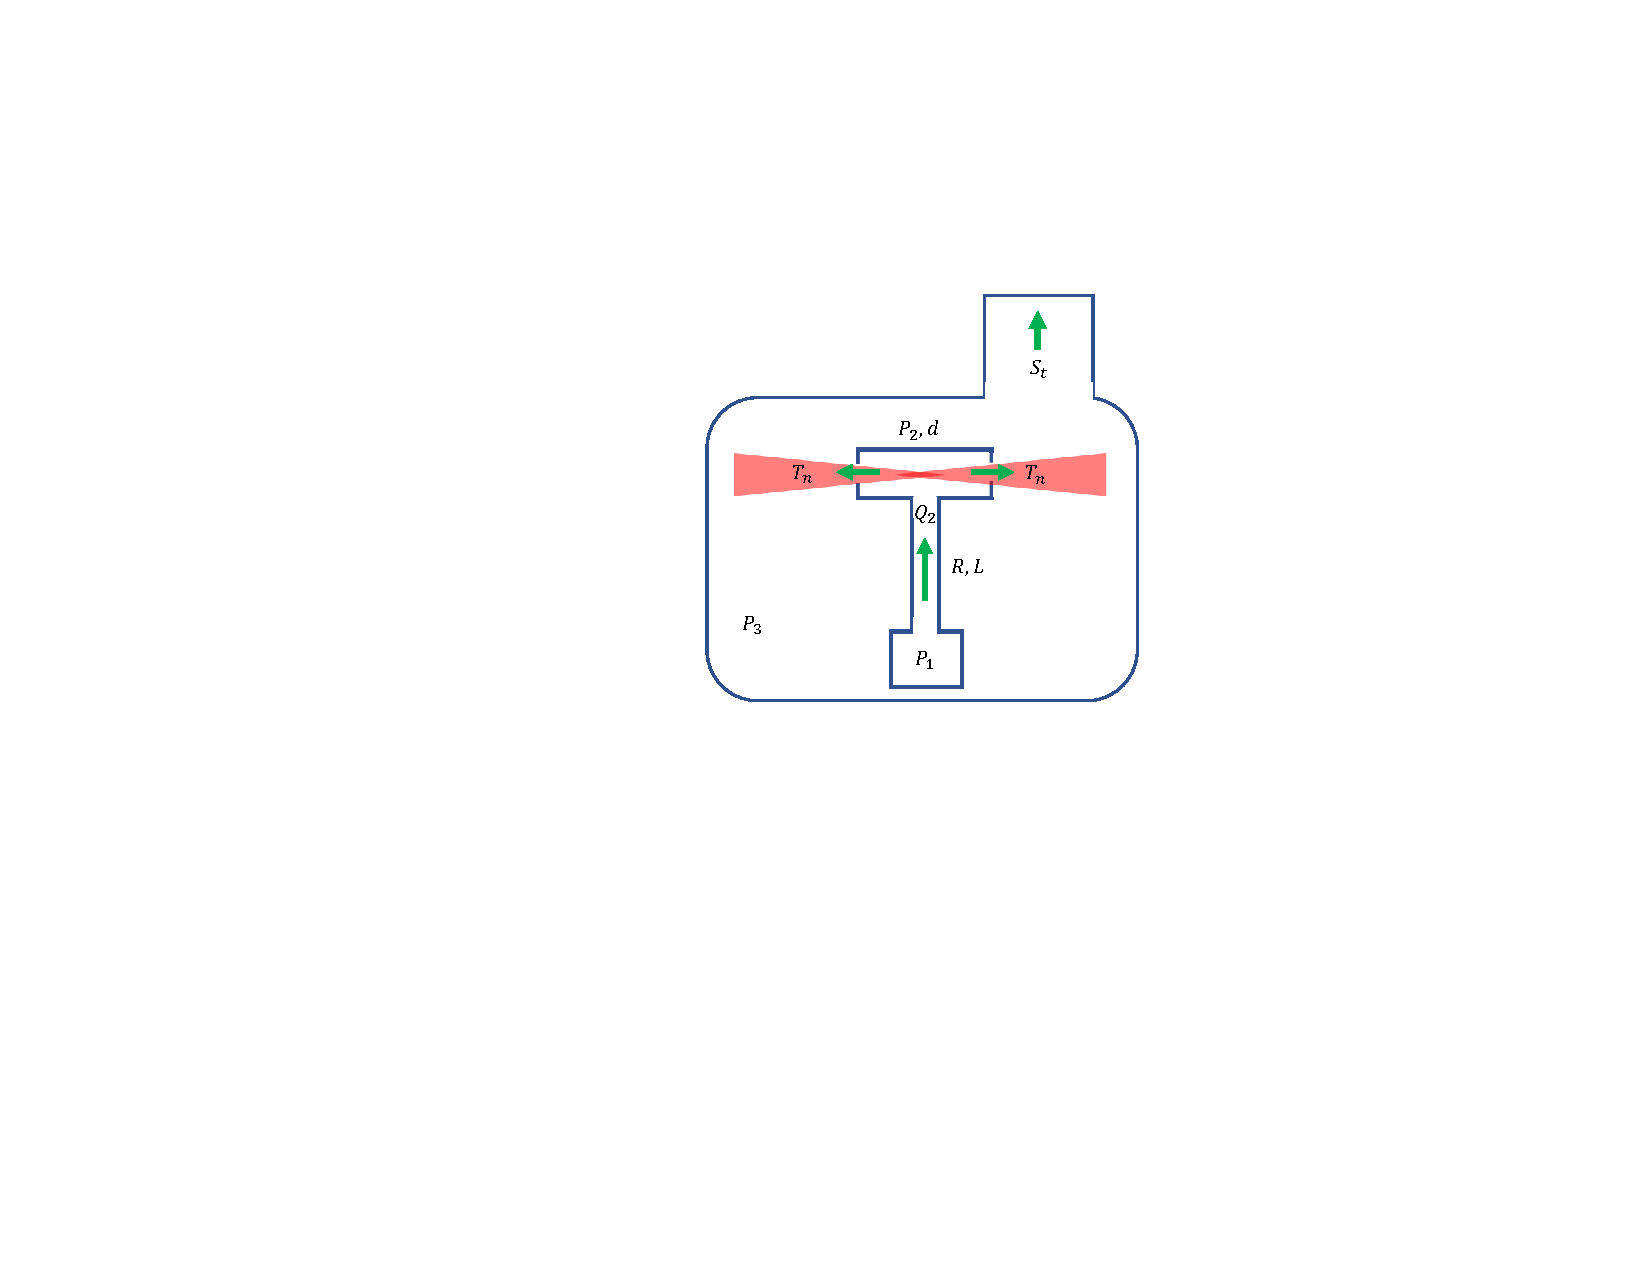
\includegraphics[width=0.75\textwidth]{figures/chap3/LPC_schematic.pdf}
	\caption{Conceptual gas flow schematic of the LPC. Arrows indicate direction of gas flow. Red shaded region indicates laser path.}
	\label{fig:LPC_schematic}
	% figure created in Chap 3 figures powerpoint.
\end{figure}

\Cref{fig:LPC_schematic} shows a gas flow model of the LPC inside the generation vacuum chamber. The green arrows indicate the direction of gas flow, and the red shaded region indicates the laser focus. The gas receiver is considered to be an infinite reservoir of gas with pressure $P_1$. This region supplies the laser interaction region with gas via a thin capillary of diameter ${R = 101.5 \ \mu \textrm{m}}$, length $L = 5 \textrm{ mm}$ and volumetric flow rate $Q_2$, modeled as an ideal isothermal gas \cite{fryerTheoryGasFlow1966,venerusLaminarCapillaryFlow2006,landauFluidMechanics2011}. The interaction region with pressure $P_2$ acts as a pressure source for two diametrically opposed supersonic gas jets \cite{millerFreeJetSources1988}, each with diameter $d$ and throughput $\hat{T}_{n}$. The generation chamber has a turbopump with pumping speed $S_{t}$ and an equilibrium pressure $P_3$. We justify this treatment by noting that we are in the supersonic regime, as $P_2 \sim 100$ Torr and $P_3 \sim 10^{-3}$ Torr. Additionally, the \textit{mean free path} $l$:
\begin{equation}
l = \frac{\mu}{P} \sqrt{\frac{\pi R T}{2 M}}
\end{equation}
is much shorter than either physical dimension ($d, W$) of the rectangular block. For helium at 100 Torr, $l \sim 1.5 \ \mu \textrm{m}$ and for argon  $l \sim 0.5 \ \mu \textrm{m}$. Therefore, we can think of the interaction region as a reservoir of gas for two diametrically opposed supersonic jets. This approach results in the following coupled equations (SI units):
\begin{align}
P_1^2 - P_2^2 &= \frac{16 \mu L Q_2 P_2}{\pi R^4}, \\
Q_2 P_2 &= 2 \hat{T}_n, \\
P_3 &= \frac{2 \hat{T}_n}{S_t}, \\
\hat{T}_n &= C P_2 d^2,
\label{eqn:LPC_coupled_equations}
\end{align}
where $C$ is the gas constant expressed in \si{m/s} (see \cref{eqn:nozzle_thruput}) and $\mu$ is the dynamic viscosity in \si{Pa.s}. Solving for the interaction pressure $P_2$ and chamber pressure $P_3$, we obtain:
\begin{align}
P_2 &= - \frac{16 C d^2 L \mu}{\pi R^4} + \sqrt{P_1^2 + \frac{256 C^2 d^4 L^2 \mu^2}{\pi^2 R^8}}, \\
P_3 &= \frac{2 C d^2}{S_t} \left( - \frac{16 C d^2 L \mu}{\pi R^4} + \sqrt{P_1^2 + \frac{256 C^2 d^4 L^2 \mu^2}{\pi^2 R^8}}  \right).
\label{eqn:LPC_pressures}
\end{align}

\begin{figure}
	\centering
	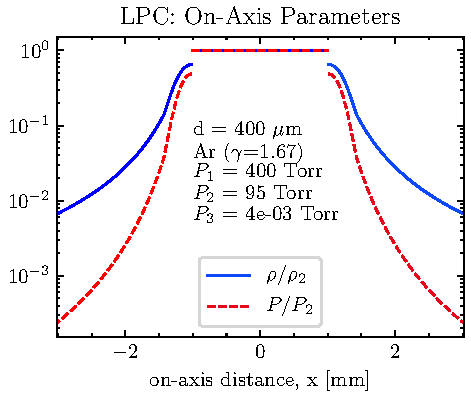
\includegraphics[width=0.75\textwidth]{figures/chap3/LPC_on_axis.pdf}
	\caption{Calculated on-axis density and pressure for the low pressure cell.}
	\label{fig:LPC_on_axis}
	% figure created in \Python Scripts\HPC\HPCvsLPC.py
\end{figure}

\Cref{eqn:mach_properties} can be used to calculate the on-axis density and pressure of the LPC, which are shown in \cref{fig:LPC_on_axis}. Our simplified model yields a constant pressure in the LPC assembly and a sharp drop off in the plume region. Note that due to the $G$ factor (see \cref{eqn:G_factor}), the FWHM of the pressure and density is simply the width of the LPC's rectangular block, $W$. When considering XUV reabsorption, we will neglect the existence of the gas plumes and treat the gas density pressure as a boxcar function with a thickness ${L_{\textrm{med}}=W}$.

\begin{figure}
	\centering
	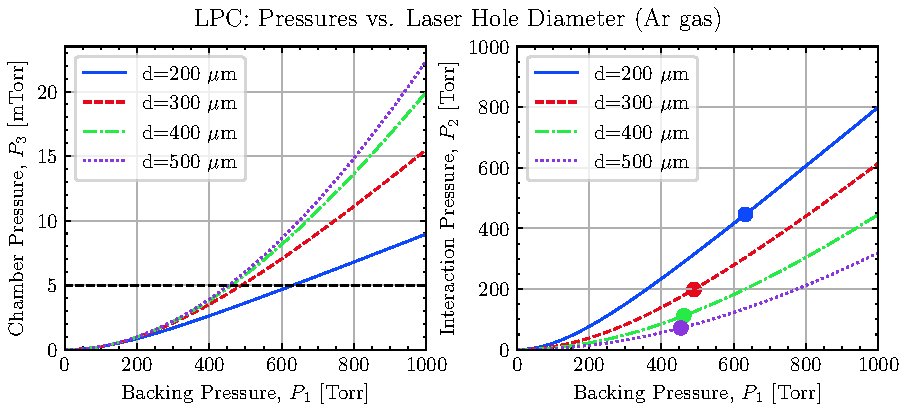
\includegraphics[width=0.9\textwidth]{figures/chap3/LPC_pressure_vs_diameter.pdf}
	\caption{Effect of the laser hole diameter $d$ on the LPC gas flow. Left panel: chamber pressure. Dashed horizontal line the indicates maximum sustainable operating pressure. Right panel: interaction pressure. Circles indicate the interaction pressure at the maximum sustainable backing pressure.}
	\label{fig:LPC_pressure_vs_diameter}
	% figure created in \Python Scripts\HPC\HPCvsLPC.py
\end{figure}

\Cref{fig:LPC_pressure_vs_diameter} shows the effect of the laser hole diameter $d$ on the chamber and interaction pressures when using argon gas. As $d$ increases relative to the capillary dimensions ($R, L$), the pressure of the interaction region decreases, and the overall conductance of the LPC assembly increases. As a result, gas is no longer efficiently trapped in the interaction region, but instead escapes out to the greater vacuum chamber. We therefore want to minimize the diameter of the laser hole as much as possible within manufacturing and optical constraints. Note that when misaligned, the laser will drill into the rectangular block, increasing the effective value of $d$ over time. For this reason, the LPC is considered a consumable part that should be replaced when its maximum operating pressure is insufficient for experimental needs.

\begin{figure}
	\centering
	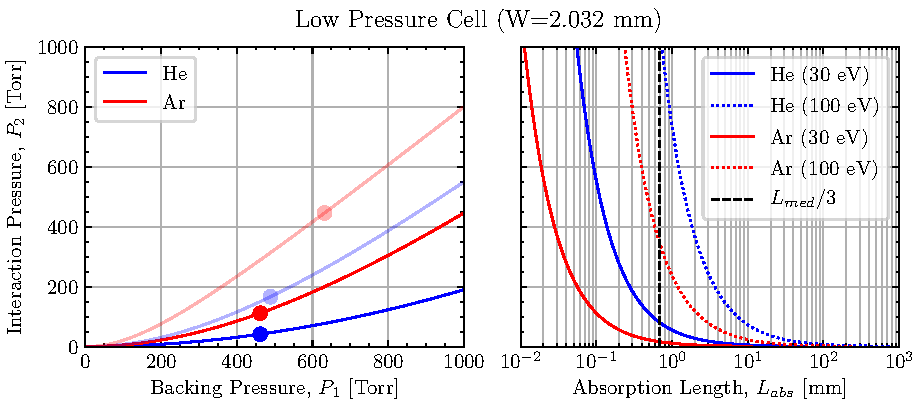
\includegraphics[width=0.9\textwidth]{figures/chap3/LPC_IntPress_AbsLen.pdf}
	\caption{Interaction pressures and XUV absorption lengths for the low pressure cell (LPC). Left panel: interaction pressure of helium (blue) and argon (red) as a function of backing pressure. Bright lines correspond to $d = 400 \ \mu$m, faint lines are for $d = 200 \ \mu$m. Right panel: absorption length for the interaction pressures shown in the left panel.}
	\label{fig:LPC_IntPress_AbsLen}
	% figure created in \Python Scripts\HPC\HPCvsLPC.py
\end{figure}

\Cref{fig:LPC_IntPress_AbsLen} shows the corresponding absorption length for a given backing and interaction pressure. In the left panel, we have selected pressure curves for $d = 400 \ \mu\textrm{m}$ (bright lines) and $d = 200 \ \mu\textrm{m}$ (faint lines) for both helium (blue) and argon (red). As in \cref{fig:LPC_pressure_vs_diameter}, the filled circles indicate the maximum sustained operating pressure before the vacuum system is overwhelmed. In the right panel, we show the corresponding absorption length $L_{\textrm{abs}}$ for low and high energy photons in both gas media. Applying the arguments of \cref{sec:XUV_reabsorption}, we compare the absorption length to the upper bound required for efficient phase matching, $L_{\textrm{abs}} = L_{\textrm{med}}/3$ (black vertical dashed line). We can see that a $200 \ \mu\textrm{m}$ LPC is capable of efficiently phase matching 100 eV photons in argon, whereas a $400 \ \mu\textrm{m}$ LPC cannot.

\subsubsection{HHG in the LPC}

To test the feasibility of the LPC for transient absorption experiments, we recorded HHG spectra under various experimental conditions.

\begin{figure}
	\centering
	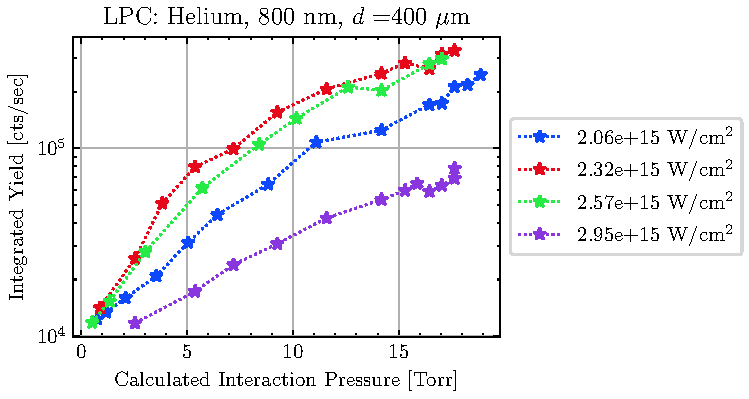
\includegraphics[width=0.90\textwidth]{figures/chap3/LPC_P_scaling_He800.pdf}
	\caption{Total harmonic yield of the LPC as a function of interaction pressure. To calculate the integrated yield, harmonic spectra are background subtracted, normalized for exposure time and integrated over the sensor area.}
	\label{fig:LPC_performance}
	% figure created in Python Scripts\HPC\LPC_800nm.py
\end{figure}

\Cref{fig:LPC_performance} shows the pressure scaling of the LPC's harmonic yield when using an {800 nm} pulse, a $f = 40 \ \textrm{cm}$ lens, and helium gas. The interaction pressure is calculated from the backing pressure and the geometry of the nozzle using \cref{eqn:LPC_pressures} using an assumed laser hole diameter of $d = 400 \ \mu$m. The pulse energy was controlled using a combination of \textit{neutral density} (ND) filters and by closing an iris before the generation chamber; average power was measured after the ND filters and before the lens using a power meter. The peak intensity was calculated assuming a 65 fs pulse duration, two 4\% transmission losses from the lens and CaF\textsubscript{2} window, and ignoring the iris-induced diffraction at the focus \cite{mahajanUniformGaussianBeams1986}. From this figure, we can see that the harmonic yield increases with increasing interaction pressure regardless of input pulse energy. Using the reabsorption model of \cref{sec:XUV_reabsorption}, this trend indicates that we are operating with a sub-optimal interaction pressure, and increasing the pressure-length would improve our harmonic yield. At the higher operating pressures, the harmonic yield is saturated when the peak intensity is $2.32 \times 10^{15}$ W/cm\textsuperscript{2}.

The red curve in \cref{fig:HHG-HPCvsLPCHPC} shows an optimized harmonic spectrum from the LPC ({17 Torr} interaction pressure, $2.32 \times 10^{15}$ W/cm\textsuperscript{2} peak intensity). Recalling \cref{sec:XUV-spectral-calibration}, a harmonic spectrum with more than an octave of bandwidth will have both $m=1$ and $m=2$ diffraction orders present on the screen. The highest resolvable harmonic is at 107 eV, which we identify as the observable cut-off energy. As such, the spectrum below 52 eV is contaminated with ${m=2}$ light and the shape of the lower energy harmonics should be ignored. From \cref{eqn:cutoff_energy}, we estimate $U_p = 26.0 \ \textrm{eV}$ and from \cref{eqn:Up-numbers}, we estimate the peak intensity to be ${I_0 = 3.5 \times 10^{14} \ \textrm{W/cm\textsuperscript{2}}}$. Both of these estimates are nearly an order of magnitude lower than the peak intensity calculated from the input pulse energy.

\begin{figure}
	\centering
	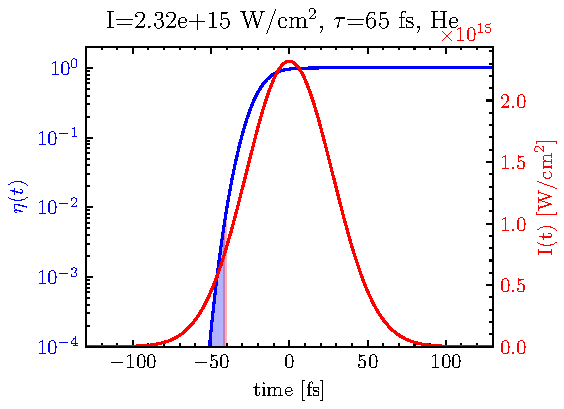
\includegraphics[width=0.75\textwidth]{figures/chap3/eta_vs_t_He800_2.32e15Wcm2.pdf}
	\caption{On-axis ionization fraction of helium (blue) and pulse envelope (red) at the focus of an 800 nm $\tau = 65$ fs, $I_0 = 2.32 \times 10^{15}$ W/cm$^2$ pulse. Times on the rising edge of the pulse where the ionization fraction is below the critical ionization fraction $\eta_c$ are shaded to indicate when harmonics are phase matched. The blue region denotes times when $\eta < \eta_c \simeq 0.55\%$ for photons with energies above 50 eV. The red region shows the additional times where lower energy ($< 50 \ \textrm{eV}$) photons can be phased matched as their critical ionization fraction is slightly higher ($\eta_c \simeq 0.7\%$).}
	\label{fig:eta_vs_t_He800_2.32e15Wcm2}
	% figure created in Python Scripts\HHG_Phasematching-master\ADK_test_updated.py
\end{figure}

\Cref{fig:eta_vs_t_He800_2.32e15Wcm2} shows the on-axis ionization fraction within a single pulse for these experimental conditions. The peak intensity is sufficiently high to completely ionize the gas medium well before the peak of the field. The on-axis ionization fraction quickly exceeds the critical ionization fraction (see \cref{fig:crit_ion_frac}) a full 50 fs before the peak of the field, as shown in the shaded regions below the blue curve. This narrow on-axis phase matching window indicates that the majority of the light is coming from the larger off-axis volume, which experiences a lower peak intensity. Nevertheless, the interaction density is too low to accommodate ideal phase matching.

Relative to the continuous free expansion gas jet, the low pressure cell has an increased interaction length but cannot reach optimal phase matching pressures. While the flux is higher than the free expansion jet, it is insufficient for an ATAS experiment.

\subsection{High Pressure Cell (HPC)}
\label{sec:HPC}

\subsubsection{Design of HPC}

The \textit{high pressure cell} (HPC) was designed to be a drop-in upgrade to the previously available HHG gas sources. As such, we did not consider a semi-infinite gas cell design which would require disruptive chamber modifications. We also did not want to implement a waveguide solution, as its performance would be strongly effected by the coupling (and therefore the laser pointing) into the assembly \cite{popmintchevExtendedPhaseMatching2008,popmintchevPhaseMatchingHigh2009}. Finally, we wanted to avoid the complications of a servicing a pulsed solenoid valve \cite{evenEvenLavieValveSource2015}, so the HPC was designed to be user-serviceable with low-cost replacement parts. As such, it consists of standard Swagelok and KF fittings with minimal modifications and a custom bellows assembly. The only consumable part is the stainless steel pipe housing the interaction region, and it only needs to be replaced when the HPC is installed or the focusing condition is changed.

\begin{figure}
	\centering
	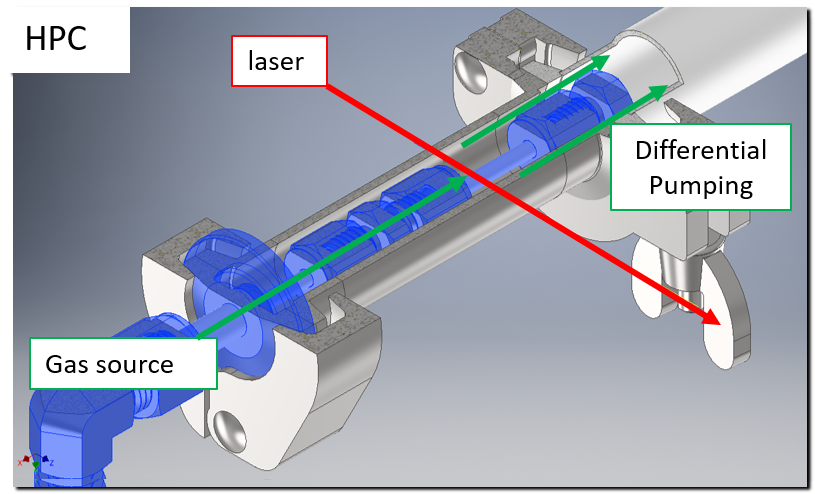
\includegraphics[width=0.9\textwidth]{figures/chap3/HPC_cutaway2.png}
	\caption{Cutaway view of the HPC interaction region. From bottom left to top right: welded gas feedthrough, concentric inner \& outer pipes, connection to edge-welded bellows. The high pressure region is shaded blue. The green lines indicate the gas flow direction; the red line indicates the laser propagation direction.}
	\label{fig:HPC_cutaway2}
\end{figure}

\begin{figure}
	\centering
	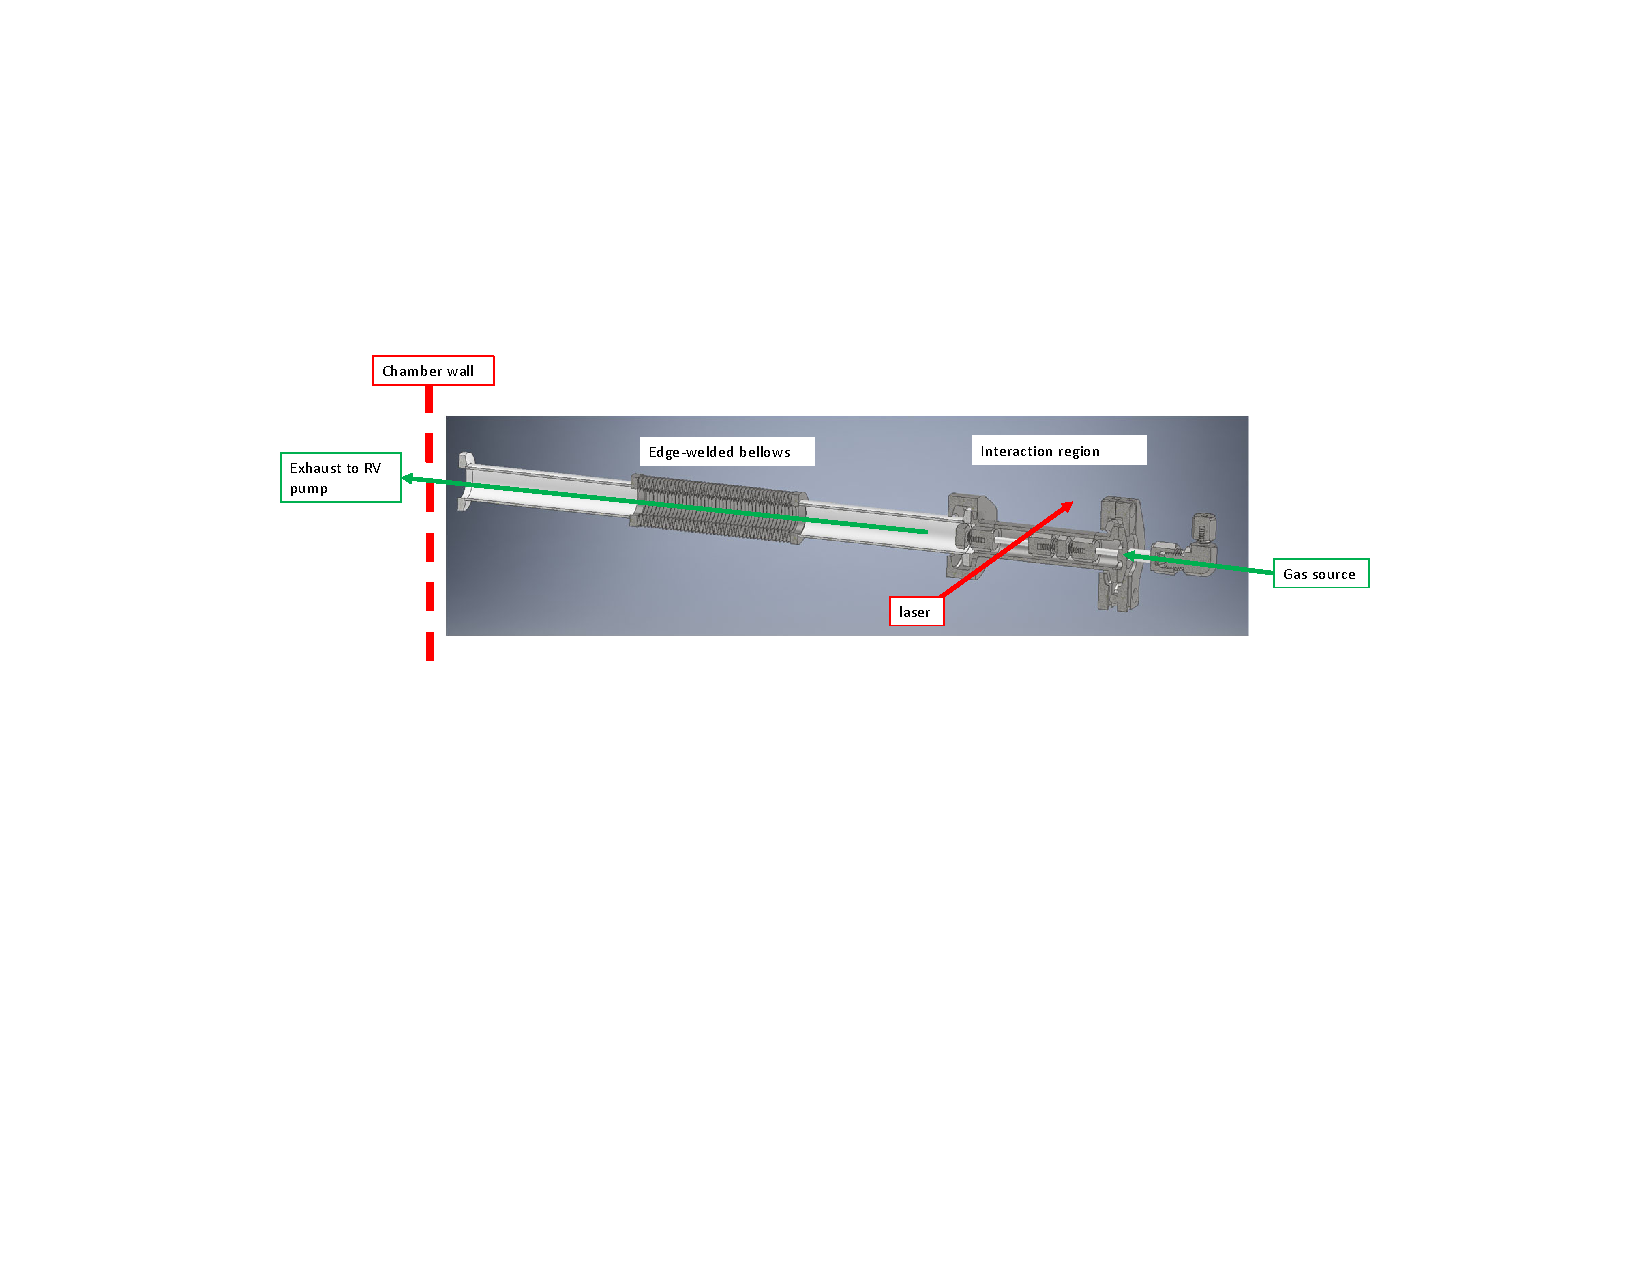
\includegraphics[width=1.0\textwidth]{figures/chap3/HPC_cutaway_bellows.pdf}
	\caption{Cutaway view of the HPC assembly showing the flexible bellows connection and connection to the chamber wall.}
	\label{fig:HPC_cutaway_bellows}
\end{figure}

The design of the HPC is shown in \cref{fig:HPC_cutaway2,fig:HPC_cutaway_bellows}. It features two concentric cylinders: a stainless steel inner pipe which serves as the interaction region and gas source, and an outer shroud connected to an external rough pump which provides differential pumping. The inner pipe is connected to a gas line with continuous flow. Laser-drilled diametrically opposed pinholes on the inner pipe wall allow for light propagation while minimizing gas flow to the outer shroud. A small portion of the gas within the outer shroud flows into the generation chamber via the machined holes, but most of the gas flows towards the exhaust and into a dedicated rough pump.

The relative positions of the inner pipe and the outer shroud are fixed by the KF hardware connections upon assembly. However, this positioning is not repeatable within the tolerances imposed by the laser transmission requirements. As a result, a new section of stainless steel pipe must be laser drilled every time the HPC is disassembled or removed from the generation chamber. The HPC assembly's position relative to the laser is adjustable via the same vacuum XYZ manipulator used for the free jet and LPC assemblies. A set of flexible bellows, visible in \cref{fig:HPC_cutaway_bellows}, allows for this movement while maintaining a vacuum-tight connection between the outer shroud and the chamber wall. A Baratron pressure gauge monitors the pressure of the KF tubing just outside the chamber wall.\footnote{Note: while the bellows can withstand an external pressure differential of 1 atm, they will become damaged if they are overpressured by 120 Torr. See \cref{app:HPC_instructions} before operating this system.} The flexible bellows has enough slack to allow the HPC to move below the optical axis, allowing the beam to pass over the top of the outer shroud. This is useful when aligning downstream optics.

The laser passes through the HPC assembly perpendicular to its symmetry axis; therefore the gas-laser interaction length is approximately equal to the diameter of the inner pipe. The outer shroud has two diametrically opposed machined 600 $\mu$m holes for the laser to pass through the assembly. During installation, the user aligns the two apertures in the outer shroud to the laser and fixes its position. Next, the inner pipe is installed and the unattenuated laser drills through the inner pipe walls. As a result, the four apertures are automatically collinear and aligned to the laser propagation axis.

\begin{figure}
	\centering
	
\includegraphics[width=0.75\textwidth]{figures/chap3/HPC_laserhole_500x370.png}
	\caption{Photograph of the HPC's inner pipe showing the laser-drilled hole (bottom center of pipe).}
	\label{fig:HPC_laserhole}
	% pictures of the HPC inner holes are located in \OneDrive - The Ohio State University\DiMauro\lab pics\HPC. The original TIFF picture was cropped with GIMP, then downsized and exported as a png.
\end{figure}

\Cref{fig:HPC_laserhole} is a photograph of the inner pipe, taken with a 0.5x telecentric lens (Edmund Optics part number 62-911). This photo shows the laser-drilled hole at the end of an experimental run. Laser drift and  misalignment, as well as daily harmonic optimization procedures over the course of several months have opened up these holes from their original diameter of approximately $100 \ \mu \textrm{m}$ to a final diameter of $430 \ \mu \textrm{m}$.

\subsubsection{Gas Flow in HPC}

\begin{figure}
	\centering
	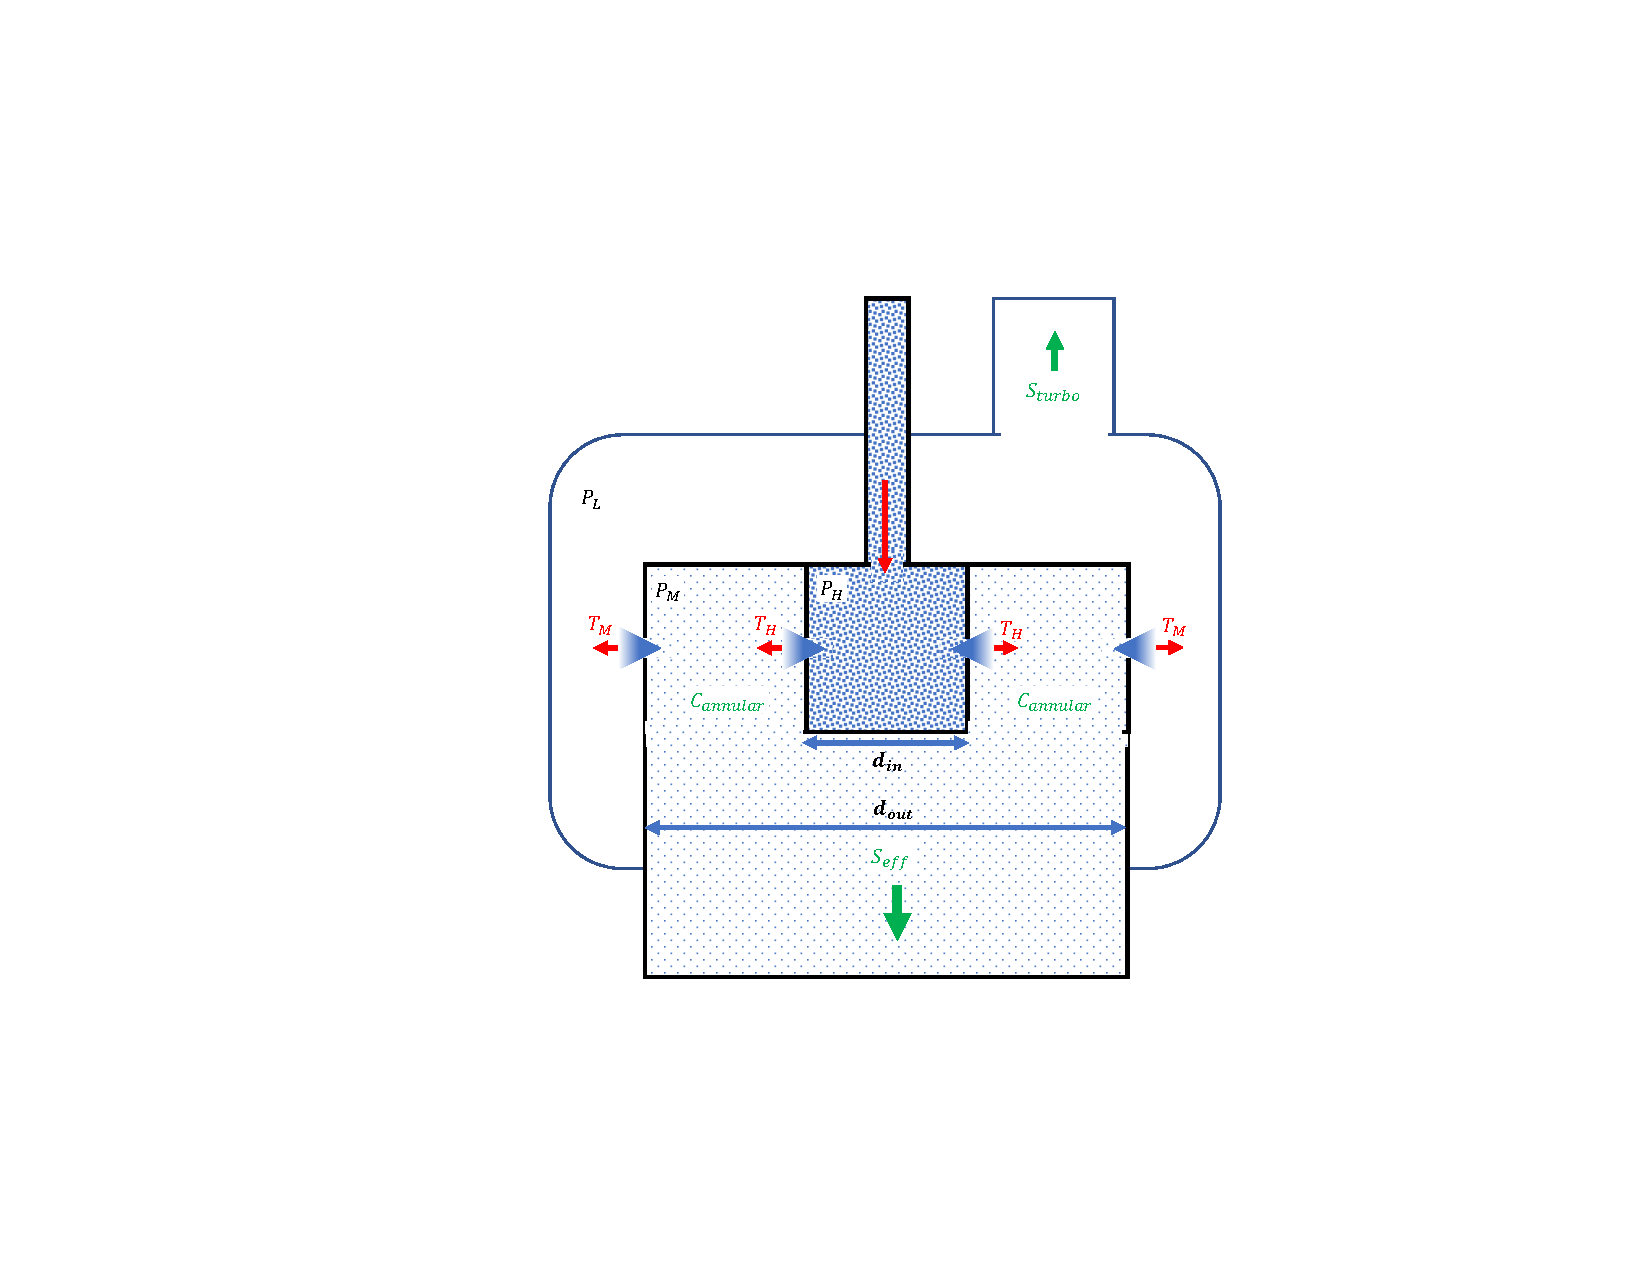
\includegraphics[width=0.75\textwidth]{figures/chap3/HPC_pressure_schematic.pdf}
	\caption{Schematic used to calculate the pressures inside the HPC and generation chamber.}
	\label{fig:HPC_pressure_schematic}
	% chap3 powerpoint
\end{figure}

The differential pumping of the HPC assembly allows the user to use much higher interaction pressures than other continuous gas sources in the DiMauro lab. In this section we will model the gas flow through the HPC to see why this is the case. \Cref{fig:HPC_pressure_schematic} shows a simplified gas flow of the HPC assembly. With the HPC cell installed, there are three distinct pressure regions within the generation chamber: the high pressure inner pipe (region $H$, with pressure $P_H$), the medium pressure outer shroud (region $M$, with pressure $P_M$), and the rest of the generation chamber remains at low pressure (region $L$, with pressure $P_L$). Two pairs of supersonic jets form at the boundaries of the three pressure regions. For each boundary, the gas jet serves as a gas sink for the higher pressure region, and as a gas source for the lower pressure region. Due to the large conductance of the tubing between the gas cylinder and the $H$ region, we treat $P_H$ as spatially constant and equal to the pressure reading on the regulator / inline pressure gauge. In the $M$ region, the majority of the gas flows orthogonal to the laser axis, down the roughing line to the floor pump; a small portion flows to the $L$ region via the machined apertures as supersonic jets. The large pressure differential (2-3 orders of magnitude) between each region justifies the assumption of supersonic flow \cite{millerFreeJetSources1988}.

In \cref{fig:HPC_pressure_schematic}, the dark blue region represents the high pressure region ($H$), the light blue region represents the medium pressure region ($M$), and the low pressure region is represented by the white region ($L$). Red arrows and text indicate gas sources, green arrows and text indicate flow towards the vacuum pumps; blue arrows and text indicate physical dimensions. $S_{\textrm{turbo}}$, $S_{\textrm{eff}}$ and $C_{\textrm{annular}}$ are the turbo pumping speed, effective rough pumping speed and annular conductance, respectively; $\hat{T}_H$ ($\hat{T}_M$) is the gas throughput from the $H$ ($M$) region into the $M$ ($L$) region from each supersonic jet.

By balancing the throughputs, we arrive at the following coupled equations:
\begin{equation}
\begin{aligned}
\hat{T}_H &= c P_H a_H^2, \\
P_M &= \frac{2(\hat{T}_H-\hat{T}_M)}{S_{\textrm{eff}}}, \\
\hat{T}_M &= c P_M a_M^2, \\
P_L &= \frac{2 \hat{T}_M}{S_{\textrm{turbo}}}.
\end{aligned}
\label{eqn:HPC-coupled-equations}
\end{equation}
In the above equations, $P_M$ and $P_L$ refer to the average background pressures in the $M$ and $L$ volumes, and the gas constant $c$ is the same as in \cref{eqn:nozzle_thruput}. That is, we ignore the structure of the plume in these calculations, which is justified because the size of each gas plume is smaller than the distance between the aperture and the next vacuum region.\footnote{For $P_H = 760 \ \textrm{Torr}$, $P_M = 0.7 \ \textrm{Torr}$ and $a_H = 100 \ \mu \textrm{m}$, $x_M = 22.1 a_H = 2.21 \ \textrm{mm}$, which is smaller than the distance between the laser drilled aperture and the outer shroud's machined aperture (6.2825 mm). For $P_L = 3 \times 10^{-4} \ \textrm{Torr}$ and $a_M = 600 \ \mu \textrm{m}$, we have $x_M = 32 a_M = 19.4 \ \textrm{mm}$, which is much smaller than the distance between the HPC and the next vacuum chamber (25 cm).} Rearranging \cref{eqn:HPC-coupled-equations}, we see that $P_M$ and $P_L$ are proportional to $P_H$, with prefactors that depend on the local effective pumping speed and aperture geometry:
\begin{equation}
\begin{aligned}
P_M &=  \frac{2 c a_H^2}{S_{\textrm{eff}}-2 c a_M^2} P_H  = \frac{S_{\textrm{turbo}}}{2 c a_M^2} P_L, \\
P_L &= \frac{4 c^2 a_M^2 a_H^2 }{S_{\textrm{turbo}} (S_{\textrm{eff}} - 2 c a_M^2)} P_H.
\end{aligned}
\label{eqn:HPC-PM-PL}
\end{equation}
The maximum achievable interaction pressure $P_H$ is only limited by the internal bellows burst pressure ($P_M \sim 120 \ \textrm{Torr}$) and the load on the turbopumps ($P_L$). From \cref{eqn:HPC-PM-PL}, we can see that we can reduce $P_M$ and $P_L$ by maximizing the effective rough pump speed $S_{\textrm{eff}}$ and minimizing the aperture sizes ($a_H$, $a_M$). The aperture sizes are set by the laser beam size and divergence, while $S_{\textrm{eff}}$ is conductance-limited by the roughing line connecting the $M$ region to the floor pump. Note that we do not need to know $S_{\textrm{eff}}$ to calculate $P_M$, provided we have accurate measurements of $a_M$ and $P_L$. However, it can be instructive to analyze how the geometry of the HPC assembly affects the effective pumping speed.

\begin{figure}
	\centering
	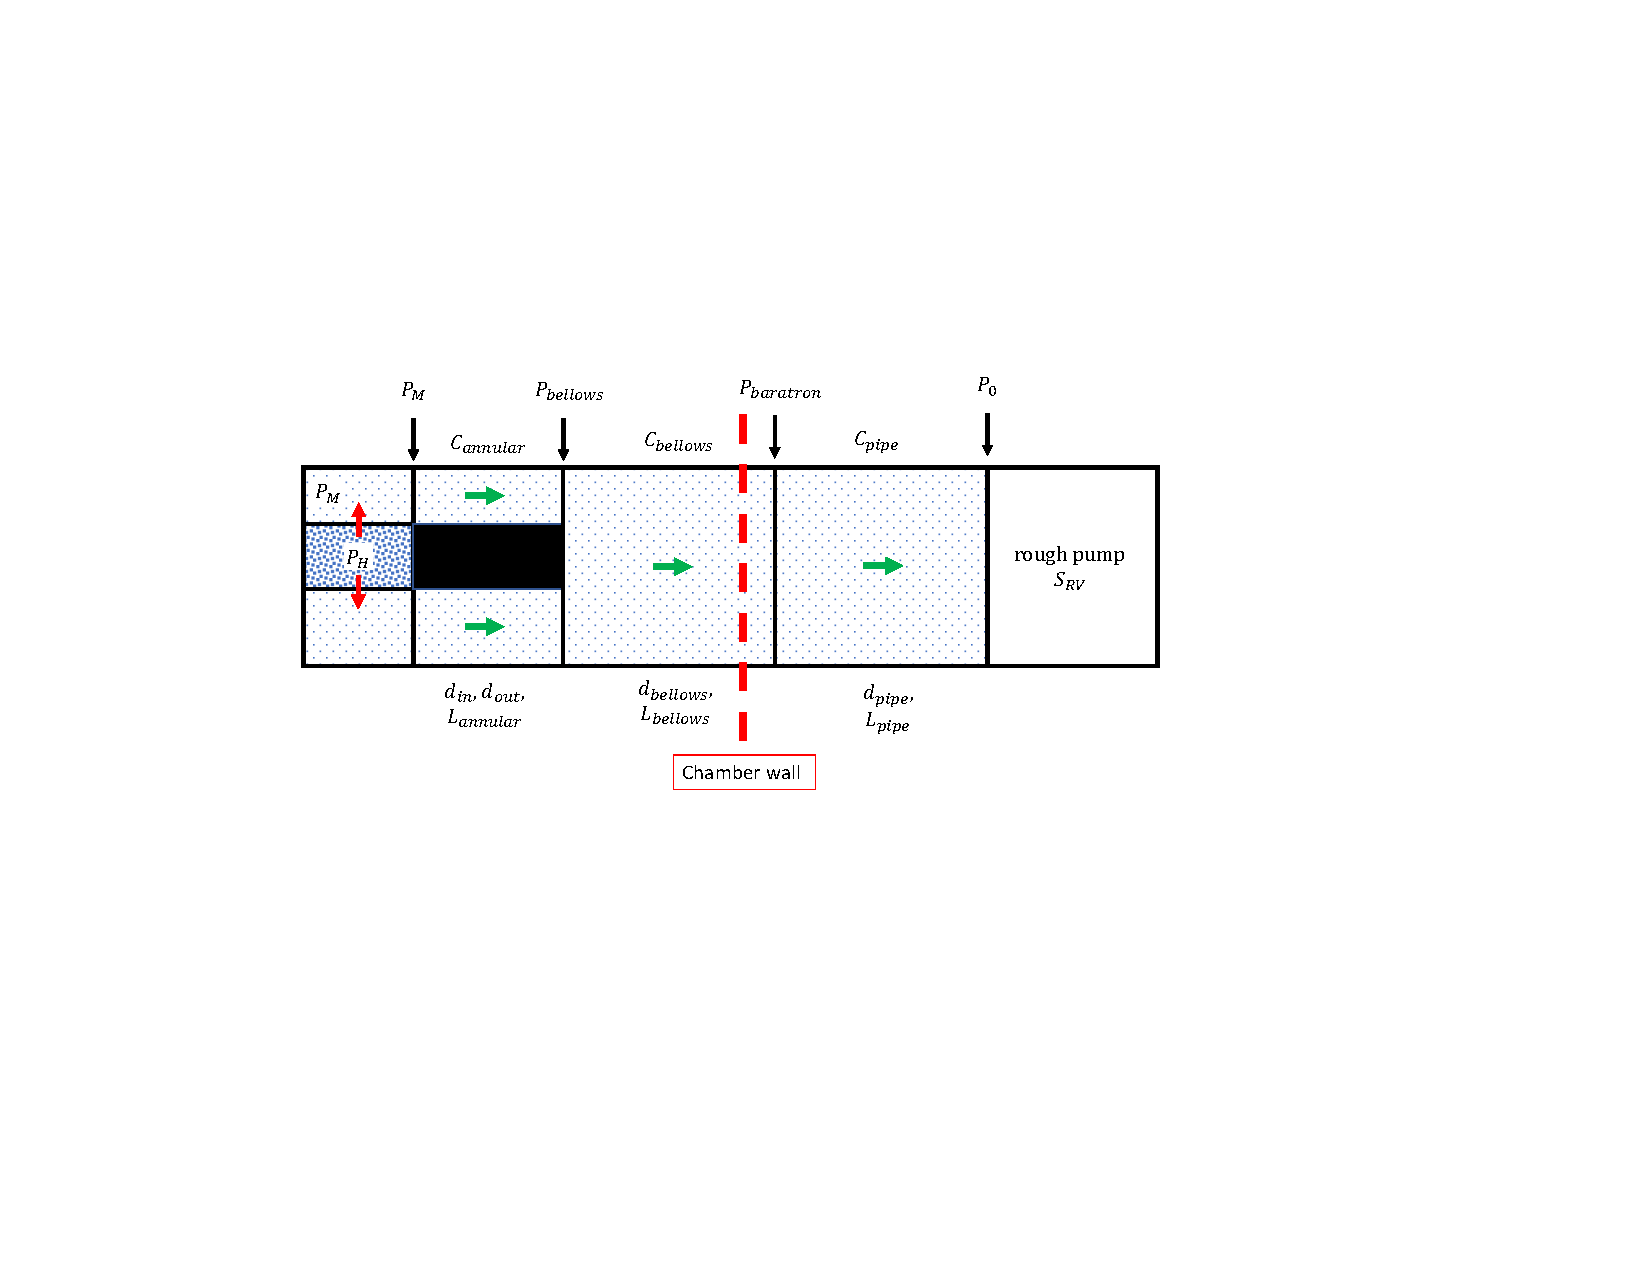
\includegraphics[width=0.9\textwidth]{figures/chap3/HPC_rough_line_schematic.pdf}
	\caption{Schematic showing the geometry and pressure profile of the HPC's rough vacuum line.}
	\label{fig:HPC_rough_line_schematic}
	% chap3 powerpoint
\end{figure}

\begin{figure}
	\centering
	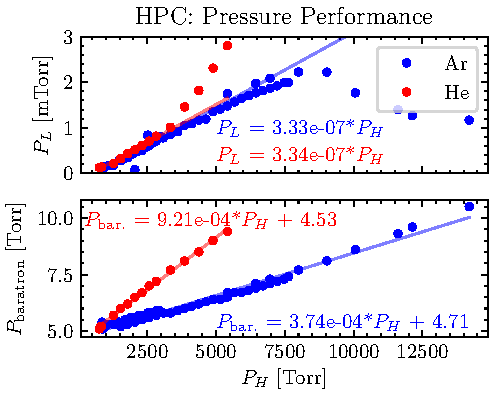
\includegraphics[width=0.75\textwidth]{figures/chap3/HPC_press_performance.pdf}
	\caption{Measured HPC pressure performance using the temporary spectroscopy station. $P_H$ is measured from the gas source's inline pressure regulator; $P_{\textrm{baratron}}$ is measured using a diaphragm gauge immediately outside the chamber wall; $P_L$ is measured using a cold cathode gauge (PTR90) and corrected using values from the manufacturer's datasheet. Linear fits to $P_{\textrm{baratron}}$ and $P_L$ are performed for  $P_H < 3000 \ \textrm{Torr}$. Regulators were changed at $P_H \sim 3000$ and $\sim 8000 \ \textrm{Torr}$, which account for the discontinuities.}
	\label{fig:HPC_press_performance}
	% chap3 powerpoint
\end{figure}

We need to make a few key assumptions before we can calculate the effective pumping speed, $S_{\textrm{eff}}$. First, we assume that the pressure in the rough line is on the order of a few Torr (this was later confirmed experimentally using the Baratron gauge). Assuming a characteristic internal length scale of $L = 1 \ \textrm{cm}$ and mean free path of ${\lambda = (5 \ \textrm{Torr}/760 \ \textrm{Torr}) \times 80 \ \textrm{nm}}$, we can calculate the \textit{Knudsen number}, $Kn = \lambda / L \sim 0.001$, which meets the criteria for continuum flow ($Kn < 0.01$). Next, assuming an effective pump speed of 5 l/s and a pipe diameter of $2 \ \textrm{cm}$, we can calculate the \textit{Reynolds number}: $Re = \rho u d / \mu \sim 1$, which meets the criteria for laminar flow ($Re < 2300$). By making reasonable assumptions, we have shown that vacuum tubing between the $M$ region and the floor pump is well within the laminar flow regime. Again, this analysis ignores the structure of the supersonic plume; the flow is likely turbulent near the boundary of the plume. The effective pumping speed in the medium pressure region $S_{\textrm{eff}}$ can therefore be calculated using standard conductance formulae for laminar flow (SI units) \cite{joustenHandbookVacuumTechnology2016}:
\begin{equation}
\begin{aligned}
\frac{1}{S_{\textrm{eff}}} &= \frac{1}{C_{\textrm{annular}}} + \frac{1}{C_{\textrm{bellows}}} + \frac{1}{C_{\textrm{pipe}}} + \frac{1}{S_{\textrm{RV}}}, \\
C_{\textrm{annular}} &= \frac{\pi}{128} \frac{1}{\eta} \frac{1}{L_{\textrm{annular}}} \left( d_{\textrm{out}}^4 - d_{\textrm{in}}^4 - \frac{(d_{\textrm{out}}^2 - d_{\textrm{in}}^2)^2}{\ln \left[d_{\textrm{out}}/d_{\textrm{in}}\right]} \right) \frac{P_M + P_{\textrm{bellows}}}{2}, \\
C_{\textrm{bellows}} &= \frac{\pi}{128} \frac{1}{\eta} \frac{d_{\textrm{bellows}}^4}{L_{\textrm{bellows}}} \frac{P_{\textrm{bellows}} + P_{\textrm{baratron}}}{2}, \\
C_{\textrm{pipe}} &= \frac{\pi}{128} \frac{1}{\eta} \frac{d_{\textrm{pipe}}^4}{L_{\textrm{pipe}}} \frac{P_{\textrm{baratron}} + P_0}{2},
\end{aligned}
\label{eqn:HPC-Seff-equations}
\end{equation}
where the pressures are measured in Pa, $\eta$ is the dynamic viscosity of the gas in Pa$\cdot$s, distances are in meters, and $S_{\textrm{RV}}$ is the rated pump speed of the floor pump in m\textsuperscript{3}/s. The geometry of the rough line system is defined in \cref{fig:HPC_rough_line_schematic}. We include in the calculation of $S_{\textrm{eff}}$ the three main vacuum elements between the outer shroud of the HPC and the floor pump:
\begin{enumerate}
	\item the short annular region formed between the inner pipe's Swagelok fittings and the inner wall of the shroud (see \cref{fig:HPC_cutaway2}), defined by inner diameter $d_{\textrm{in}} = 1.283 \ \textrm{cm}$, outer diameter $d_{\textrm{out}} = 1.575 \ \textrm{cm}$, length $L_{\textrm{annular}} = 2 \ \textrm{cm}$, entrance pressure $P_M$ and exit pressure $P_{\textrm{bellows}}$;
	\item the edge-welded bellows assembly, defined by length $L_{\textrm{bellows}} = 27.6 \ \textrm{cm}$, interior diameter $d_{\textrm{bellows}} = 1.7272 \ \textrm{cm}$, entrance pressure $P_{\textrm{bellows}}$ and exit pressure $P_{\textrm{baratron}}$;
	\item the length of flexible PVC pipe connecting the exterior of the chamber to the floor pump, defined by length $L_{\textrm{pipe}} = 150 \ \textrm{cm}$ and interior diameter $d_{\textrm{pipe}} = 2 \ \textrm{cm}$, entrance pressure $P_{\textrm{baratron}}$ and exit pressure $P_0$.
\end{enumerate}

Given the above dimensions, the annular region has an outsized impact on the total conductance of the differential pumping system:
\begin{equation*}
\begin{aligned}
C_{\textrm{annular}} &= (5.83 \times 10^{-10} \ \textrm{m}^{3}) \times (\bar{p}_{\textrm{annular}}/\eta), \\
C_{\textrm{bellows}} &= (7.91 \times 10^{-9} \ \textrm{m}^{3}) \times (\bar{p}_{\textrm{bellows}}/\eta), \\
C_{\textrm{pipe}} &= (2.62 \times 10^{-9} \ \textrm{m}^{3}) \times (\bar{p}_{\textrm{pipe}}/\eta),
\end{aligned}
\end{equation*}
where $\bar{p}_i$ is the average pressure in each element. For a floor pump speed with ${S_{\textrm{RV}} = 5 - 11 \ \textrm{l/s}}$, the effective pump speed $S_{\textrm{eff}}$ in the $M$ region will be between 20\% and 88\% of $S_{\textrm{RV}}$, assuming a constant average pressure $\bar{p}$ in the range ${1 - 30 \ \textrm{Torr}}$.

The HPC was initially tested in a simplified vacuum system, called the \textit{temporary spectroscopy station}, as the TABLe's interferometer was being used by another graduate student at the time. The temporary spectroscopy station consisted of the TABLe's target chamber (repurposed as a generation chamber) connected to the photon spectrometer via a differential pumping chamber. There was no XUV refocusing optic. Instead of using the TABLe's high throughput RV system (see \cref{fig:rough_vacuum_schematic}), individual floor pumps to back the turbos. The generation turbo was backed by a Leybold D40B ($S_{\textrm{RV}} = 13.3 \ \textrm{l/s}$); the HPC rough line was pumped by a scroll pump ($S_{\textrm{RV}} \sim 10 \ \textrm{l/s}$), and two smaller Leybold D16B pumps ($S_{\textrm{RV}} = 5.5 \ \textrm{l/s}$) were used to back the differential and photon spectrometer turbos.

\begin{figure}
	\centering
	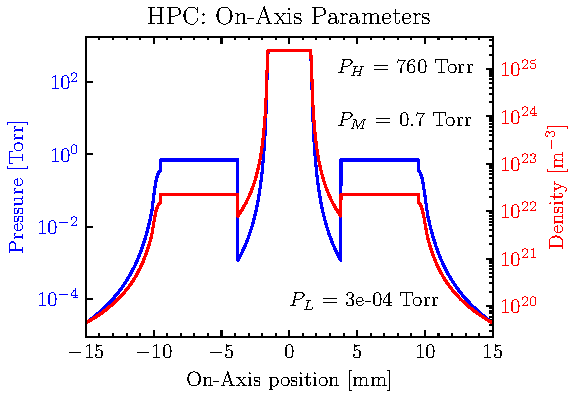
\includegraphics[width=0.75\textwidth]{figures/chap3/HPC_on-axis-pressure.pdf}
	\caption{Calculated on-axis pressure and density profiles for helium with $P_H = 760$ Torr, $P_M = 0.7$ Torr and $P_L = 3 \times 10^{-4}$ Torr.}
	\label{fig:HPC_on-axis-pressure}
	% plot made in \Python Scripts\HPC\HPCvsLPC.py
\end{figure}

\Cref{fig:HPC_press_performance} shows the HPC's pressure performance for helium and argon gas as measured in the temporary spectroscopy station. Pressures were measured with a Baratron diaphragm gauge ($P_{\textrm{baratron}}$, located immediately outside the chamber wall) and a Leybold PTR90 cold cathode gauge ($P_L$, attached to the generation chamber). The pressure readings from the cold cathode gauge are corrected using the manufacturer's datasheet; the Baratron's readings are gas species-independent. Here, we see that $P_{\textrm{baratron}}$, which is approximately equal to $P_M$, scales linearly with respect to the backing pressure $P_H$ over a wide range of pressures. Note that the slope for helium is approximately 3 times that for argon, which is consistent with their gas constants ($c=14 \ \textrm{l/cm}^2\textrm{/s}$ for Ar, $c=45 \ \textrm{l/cm}^2\textrm{/s}$ for He).

Turning our attention the chamber pressure ($P_L$), we see a rollover in argon around $P_H \sim 8000 \ \textrm{Torr}$, and in helium we see a discontinuity in the slope at $P_H \sim 3000 \ \textrm{Torr}$. These features are unphysical and are likely caused by the cold cathode gauge malfunctions. Regardless, we can see that the chamber pressure stays in the milliTorr regime even when $P_H \simeq 5,000$ Torr for helium and $P_H \simeq 14,000$ Torr for argon.

\begin{figure}
	\centering
	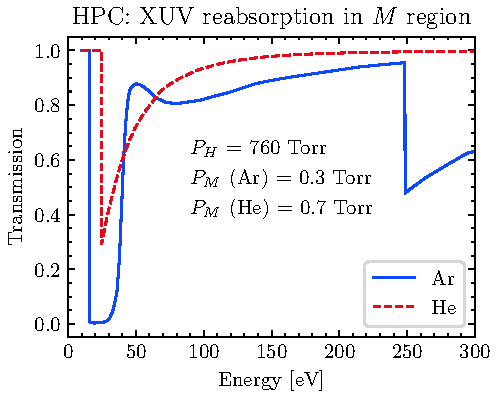
\includegraphics[width=0.75\textwidth]{figures/chap3/HPC_absorption.pdf}
	\caption{Expected XUV reabsorption in the $P_M$ region for different generating media. $P_M$ calculated using $P_H = 760 \ \textrm{Torr}$ via \cref{eqn:HPC-PM-PL}. Absorption data from \cite{gulliksonCXROXRayInteractions}.}
	\label{fig:HPC_absorption}
	% plot made in \Python Scripts\CXRO\test\CXRO.py or \HPCvsLPC.py
\end{figure}

\Cref{fig:HPC_on-axis-pressure} shows the calculated on-axis density and pressure profile of the HPC for helium and an interaction pressure of 760 Torr. The intermediate pressure $P_M$ is assumed to be equal to $P_{\textrm{baratron}}$ and is calculated using the linear coefficient obtained in \cref{fig:HPC_press_performance}. In calculating $P_M$, we omit the offset of $4.53 \ \textrm{Torr}$ which is a measurement artifact of the Baratron gauge. The on-axis pressure shows that there is a non-negligible amount of gas in the $M$ region, which is several millimeters long. If we assume that HHG occurs solely in the $H$ region, then XUV flux may inadvertently be reabsorbed when propagating through the $M$ region.

\begin{figure}
	\centering
	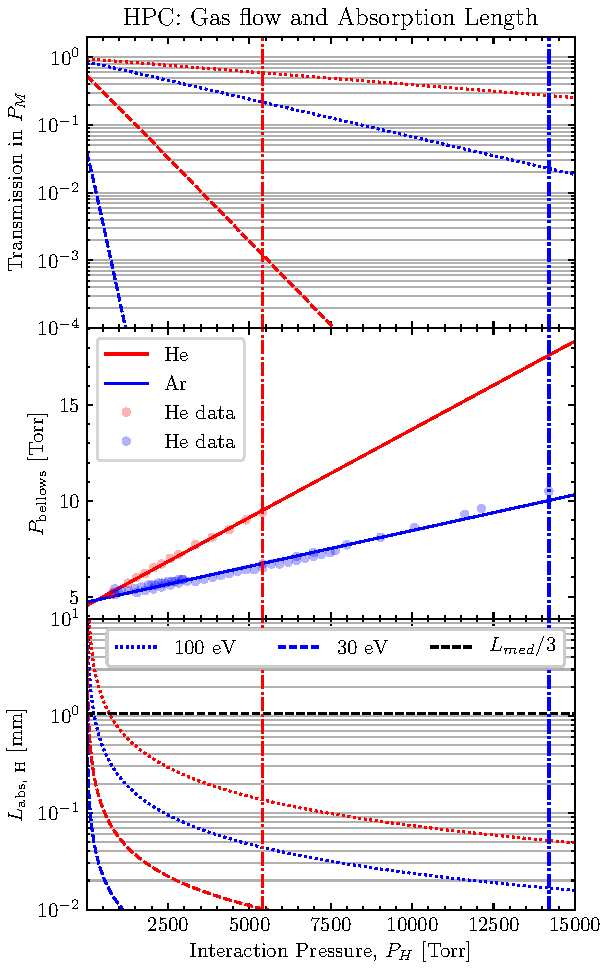
\includegraphics[width=0.75\textwidth]{figures/chap3/HPC-gas-flow-int-length.pdf}
	\caption{HPC calculated performance as a function of interaction pressure, assuming $a_H = 100 \ \mu \textrm{m}$ and the fit from in \cref{fig:HPC_press_performance}. For both panels, blue (red) lines correspond to argon (helium), dashed (dotted) lines correspond to 30 (100) eV photons. Vertical dashed lines indicate the highest experimentally achieved pressures.}
	\label{fig:HPC-gas-flow-int-length}
	% plot made in \Python Scripts\CXRO\test\CXRO.py or \HPCvsLPC.py
\end{figure}

\Cref{fig:HPC_absorption} estimates the XUV transmission (via $T = \int_M \dd{z} \exp (- \rho(z) \mu_a z )$) in the $M$ region assuming the aforementioned pressure profile, and \cref{fig:HPC-gas-flow-int-length} shows the XUV transmission in the $M$ region for 30 and 100 eV photons over a range of pressures. In both figures, XUV absorption in the $L$ region is neglected due to its low pressure. \Cref{fig:HPC-gas-flow-int-length} also compares the absorption length ($L_{\textrm{abs}} = 1 / \rho \mu_a$) to the medium length $L_{\textrm{med}}$. We can see that the HPC can reach sufficiently high interaction pressures and length to meet the phase matching guidelines laid out in \cref{sec:XUV_reabsorption}.

\subsubsection{HHG in the HPC}

An effort was made to increase the XUV flux in the energy range 90 - 130 eV, which would allow the measurement of the Si $L$-edge in an ATAS experiment. To this end, HHG experiments were performed in the temporary spectroscopy station using the HPC and an $f = 40 \ \textrm{cm}$ CaF\textsubscript{2} lens. Input power and phase matching were simultaneously controlled using an adjustable aperture located before the focusing optic. The interaction pressure was controlled with the gas cylinder's regulator and measured using an inline digital pressure gauge (Ashcroft model 2274). The fundamental and $<50$ eV harmonics were blocked using a $200 \ \mu\textrm{m}$ Zr filter located approximately $75 \ \textrm{cm}$ downstream of the HPC. The spectrometer's energy axis was crudely calibrated by counting the harmonics above the Al $L$-edge and assuming $2\omega_1$ spacing, and fitting to a \nth{5} degree polynomial (see \cref{sec:XUV-spectral-calibration}), and all HHG yields shown are scaled by the Jacobian. To isolate the effects of pressure scaling, phase matching conditions were optimized at low pressure and held constant as the interaction pressure was controlled. To maximize harmonic flux, the HPC's position relative to the focus was optimized (at the focus for helium and downstream of the focus for argon). Phase matching conditions were optimized for photon energies above 100 eV. Pulse energy was measured using a power meter immediately before the generation chamber; the reported values do not take into account any transmission losses of the fundamental due to the two HPC vacuum apertures between the generation chamber's window and the interaction region ($H$). Calculating the interaction intensity is complicated by diffraction and transmission losses resulting from the HPC's apertures; we report the intensities that would occur in the absence of the HPC assembly with the caveat that the actual intensities are likely lower.

\begin{figure}
	\centering
	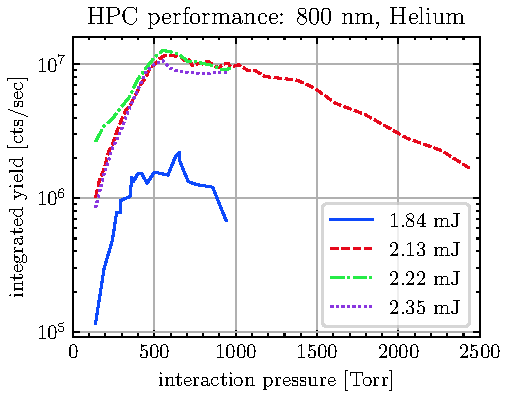
\includegraphics[width=0.75\textwidth]{figures/chap3/HPC_P_scaling_He800.pdf}
	\caption{Total harmonic yield as function of interaction pressure in the HPC. To calculate the integrated yield, harmonic spectra are background subtracted, normalized for exposure time and integrated over the sensor area (divergence and energy).}
	\label{fig:HPC_P_scaling_He800}
	% plot made in \Python Scripts\HPC\HPC_800nm.py
\end{figure}

The total harmonic yield for helium using 800 nm light as a function of interaction pressure is shown in \cref{fig:HPC_P_scaling_He800}. Unlike the LPC, we can see a maximum in the harmonic yield with respect to interaction pressure, indicating that we are no longer limited by the vacuum performance of the gas source. The total yield is maximized for $P_H \sim 600 \ \textrm{Torr}$. Helium's high ionization potential ($I_p = 24.5874 \ \textrm{eV}$) necessitates high laser intensities to efficiently drive the HHG process, and we see that a $\simeq 0.36 \times 10^{15}$ W/cm\textsuperscript{2} increase in peak intensity increases total harmonic yield by nearly an order of magnitude. In contrast to the LPC, where we saw a saturation in harmonic yield at around $\simeq 2.32 \times 10^{15}$ W/cm\textsuperscript{2}, the HPC's yield does not saturate until $\simeq 2.67 \times 10^{15}$ W/cm\textsuperscript{2}. This is likely due to the lower transmission of the HPC's vacuum apertures, estimated at $\simeq 90 \%$. In the following discussion we report the normalized yield, which is obtained by background subtracting, integrating over the spatial dimension of the sensor, and normalizing by integration time. In the event that multiple spectra are obtained for identical conditions, we average the results together.

\begin{figure}
	\centering
	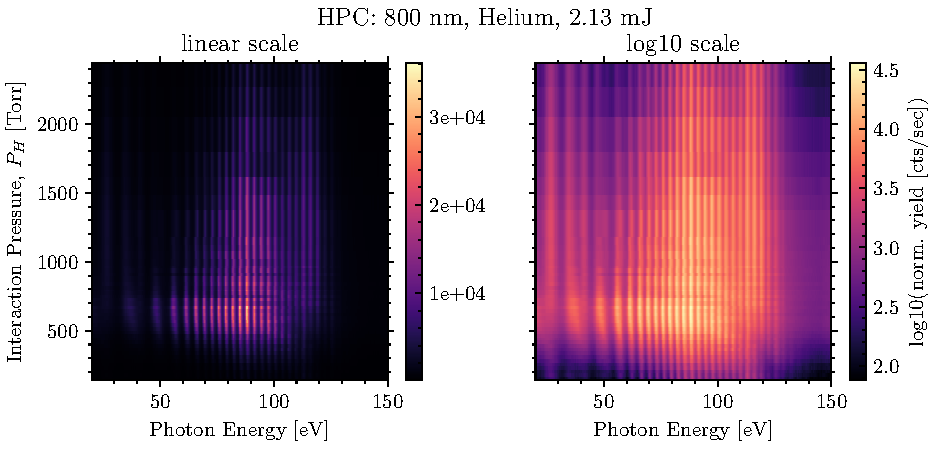
\includegraphics[width=0.9\textwidth]{figures/chap3/HPC_800nm_He_spectrogram.pdf}
	\caption{Harmonics generated from helium as a function of interaction pressure for $\lambda_1 = 800 \ \textrm{nm}$, a peak intensity of $2.67 \times 10^{15}$ W/cm\textsuperscript{2} and a $200 \ \mu \textrm{m}$ Zr filter. Note that different energy harmonics are phase matched at different pressures. To calculate the integrated yield, harmonic spectra are background subtracted, normalized for exposure time and integrated over the sensor area.}
	\label{fig:HPC_800nm_He_spectrogram}
	% plot made in \Python Scripts\HPC\HPC_800nm.py
\end{figure}

\Cref{fig:HPC_800nm_He_spectrogram} shows a spectrogram of the 800 nm $2.67 \times 10^{15}$ W/cm\textsuperscript{2} helium dataset. We can see a broad maximum in yield for energies below $\sim 100 \ \textrm{eV}$ below $650 \ \textrm{Torr}$. Harmonic yield above 100 eV is maximized above $700 \ \textrm{Torr}$ at the expense of lower energy light; light below 80 eV is suppressed when $P_H > 1600 \ \textrm{Torr}$. This observed dispersion matches the general $1/\Delta n$ pressure scaling in \cref{fig:recip_deltan_plot} and the absorption in \cref{fig:HPC-gas-flow-int-length}.

\begin{figure}
	\centering
	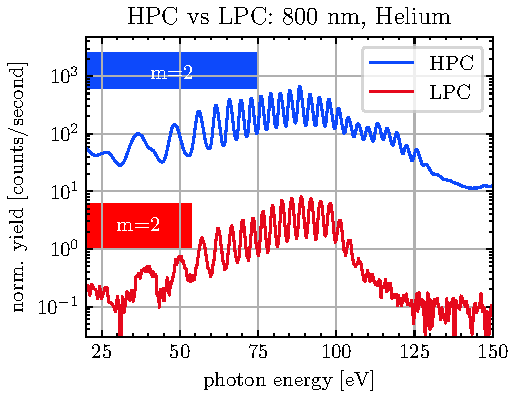
\includegraphics[width=0.75\textwidth]{figures/chap3/HPC_vs_LPC_800He.pdf}
	\caption{Comparison of the LPC and the HPC in helium at 800 nm. Generation conditions for each were optimized (LPC: 17 Torr interaction pressure, $2.32\times10^{15}$ W/cm\textsuperscript{2}; HPC: 650 Torr, $2.67 \times 10^{15}$ W/cm\textsuperscript{2}) in helium at 800 nm. The higher interaction pressure extends the phase matched region from $ \sim 110 \ \textrm{eV}$ to $\sim 130 \ \textrm{eV}$, and increased pressure-length product increases the XUV brightness by at least two orders of magnitude across the spectrum. Note that harmonics with energies less than half the cutoff are contaminated by \nth{2} order diffraction from the XUV spectrometer's grating. Faint blue line removes the calculated absorption losses in the medium pressure ($M$) region. Normalized yield is calculated by background subtracting the 2D spectra, integrating the spatial dimension of the sensor, normalizing by exposure time and applying the Jacobian.}
	\label{fig:HHG-HPCvsLPCHPC}
	% plot made in \Python Scripts\HPC\HPCvLPC_comparison.py
\end{figure}

\Cref{fig:HHG-HPCvsLPCHPC} compares the spectra of the LPC and the HPC. The portion of the sensor that is contaminated with $m=2$ XUV light (lower half of the spectra) is indicated by a red or blue box. Other than the gas source, these datasets were taken under identical circumstances\footnote{Nominal differences in pulse energy are attributed to lower MIR transmission of the HPC's apertures. Both experiments were conducted at the threshold of saturation intensity.}, so we can compare their spectral amplitudes. We can see that the total harmonic yield of the HPC exceeds that of the LPC by about two orders of magnitude. Additionally, the highest observable harmonic is increased from $\sim 110$ eV to $\sim 130$ eV.  Taking into account the calculated pressure profile in the $M$ region and the photoabsorption cross section of helium, we plot the absorption-free yield ($P_M =0$) in faint blue.

\begin{figure}
	\centering
	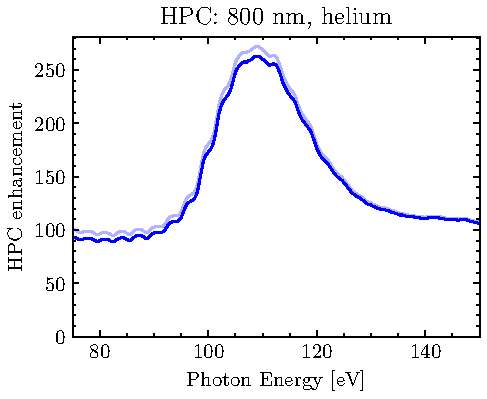
\includegraphics[width=0.75\textwidth]{figures/chap3/HPC_He800nm_enhancement.pdf}
	\caption{Relative performance of the HPC compared to the LPC in the energy range 75 - 150 eV. Faint blue line includes the calculated transmission factor in the $M$ region. Datasets are the same as in \cref{fig:HHG-HPCvsLPCHPC}.}
	\label{fig:HPC_He800nm_enhancement}
	% plot made in \Python Scripts\HPC\HPCvLPC_comparison.py
\end{figure}

\Cref{fig:HPC_He800nm_enhancement} shows the relative enhancement of HHG using the HPC compared to the LPC. Over the energy range 75 - 150 eV, we can see a 50 - 60x improvement in yield, with a $\sim 150 \textrm{x}$ enhancement centered at 110 eV. The position of this enhancement peak is very sensitive to generation conditions and can be shifted by tens of eV by adjusting the iris.

We can compare the measured performance to what was expected from our previous discussions on HHG. From \cref{eqn:HHG_Nout_2}, we expect the harmonic yield to scale as $(PL_{\textrm{med}})^2$, and when considering the pressure models developed above, we would expect the HPC to outperform the LPC by a factor of roughly 3500. After taking into account the XUV absorption in the $M$ region, we measured a factor of 150, which is significantly less than the expected value. This discrepancy (factor of $\sim 23$) may be attributed to a smaller effective MIR spot size and a diffraction-induced non-Gaussian beam shape at the focus. The higher interaction pressures may result in an ionization-induced defocusing of the fundamental beam, lowering the interaction intensity and therefore the harmonic yield \cite{altucciInfluenceAtomicDensity1996}.

\begin{figure}
	\centering
	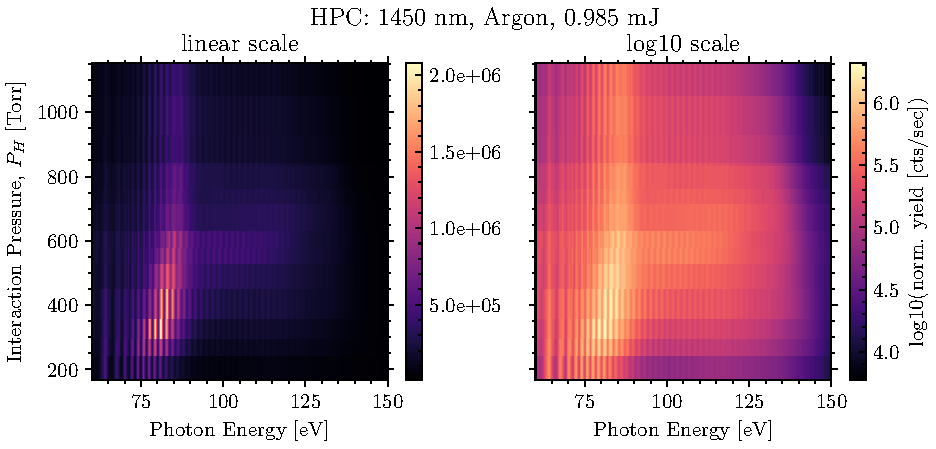
\includegraphics[width=0.9\textwidth]{figures/chap3/HPC_1450nm_Ar_spectrogram.pdf}
	\caption{Performance of the HPC using argon at 1450 nm. Normalized yield is calculated by background subtracting the 2D spectra, integrating the spatial dimension of the sensor, normalizing by exposure time and applying the Jacobian.}
	\label{fig:HPC_1450nm_Ar_spectrogram}
	% plot made in \Python Scripts\HPC\HPC_Ar_signal.py
\end{figure}

Similar experiments were performed using argon using signal wavelengths. \Cref{fig:HPC_1450nm_Ar_spectrogram} shows a spectrogram of argon's harmonic yield at 1450 nm under typical operating conditions. Note that the lower ionization energy ($I_P = 15.75962 \ \textrm{eV}$) translates into a lower peak intensity for optimal harmonic generation. We observe a rolling maximum in the harmonic yield, from 70 to 90 eV, as the interaction pressure is increased from 200 to 600 Torr. At higher energies ($> 90 \ \textrm{eV}$), we see a broad maximum between 250 and 850 Torr. As the pressure increases past 850 Torr, harmonic yield uniformly decreases.

\begin{figure}
	\centering
	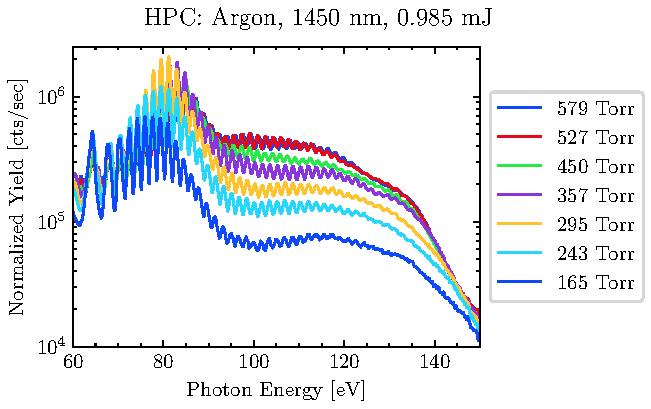
\includegraphics[width=0.9\textwidth]{figures/chap3/HPC_1450nm_Ar_lineouts.pdf}
	\caption{Spectral lineouts of \cref{fig:HPC_1450nm_Ar_spectrogram} for pressures below the maximum in harmonic yield. Normalized yield is calculated by background subtracting the 2D spectra, integrating the spatial dimension of the sensor, normalizing by exposure time and applying the Jacobian.}
	\label{fig:HPC_1450nm_Ar_lineouts}
	% plot made in \Python Scripts\HPC\HPC_Ar_signal.py
\end{figure}

\Cref{fig:HPC_1450nm_Ar_lineouts} shows spectral lineouts of \cref{fig:HPC_1450nm_Ar_spectrogram} for lower interaction pressures. In this figure, we see that the harmonic yield above 90 eV increases about an order of magnitude as the interaction pressure is increased from 165 to 527 Torr, which is perfectly in line with the expected $P^2$ scaling ($527^2/165^2 = 10.2$). At 450 Torr and above, we observe a blueshifting of the harmonic comb, which is suggestive that the fundamental is experiencing nonlinear propagation effects near the focus. This effect was not observed in helium, which has a significantly higher ionization potential.

Although we do not have a directly comparable LPC HHG dataset, we can make some general comparisons between the two gas sources. Recalling \cref{fig:LPC_IntPress_AbsLen}, the LPC is limited to a maximum interaction pressure of between 50 and 175 Torr (depending on laser aperture size). If HHG follows the observed $P^2$ scaling, then the HPC would be between 9 and 110 times brighter than the LPC if both systems are optimized for maximum HHG yield.

We note that the increased XUV absorption of argon results in a lower overall enhancement factor than for helium \cite{popmintchevPhaseMatchingHigh2009}. The pressure model developed above predicts an XUV transmission between 85 and 90\% for $P_H = 527 \ \textrm{Torr}$ for photon energies between 75 and 150 eV.

We observe that at 100 eV, the optimized 1450 nm Ar dataset is $\sim 3\textrm{x}$ brighter than the 800 nm He dataset, despite being at performed at a longer wavelength. Assuming $\lambda^{-4}$ scaling of the yield at a single harmonic (see \cref{sec:HHG_propagation_recombination}), we lose a factor of $\sim 10$ in yield by increasing from 800 to 1450 nm. Therefore, for optimized generation conditions using the same fundamental wavelength, we should expect Ar to be 30x brighter than He at a given photon energy $\dd E$.

\subsection{Pulsed Amsterdam Piezo Valve}
% piezovalve yield vs pressure: C:\testdata\2019_10_10

We can reduce the gas load on the turbopumps while achieving a moderately high interaction pressure by using a pulsed gas source, as the gas throughput scales approximately with the valve's duty cycle \cite{christenStationaryFlowConditions2013}. Typical valve opening times are on the order of tens of microseconds \cite{irimiaSituCharacterizationCold2009,mengMeasurementDensityProfile2015,irimiaShortPulseMicrosecond2009}, which results in a duty cycle of $1 - 10 \%$ percent when operating at 1 kHz. Commercially available valve designs consist of either a plunger-solenoid \cite{evenEvenLavieValveSource2015} or a piezoelectric flapper \cite{irimiaSituCharacterizationCold2009,mengMeasurementDensityProfile2015,irimiaShortPulseMicrosecond2009}.

In our experience the plunger-solenoid design is prone to mechanical failure, which necessitates the device be sent back to the manufacturer for repairs. Unfortunately, it is not uncommon to experience months of equipment downtime during these regular service events. For this reason, we eschewed the use of a plunger-solenoid valve in favor of a simpler CW gas delivery solution when designing the beamline.

\begin{figure}
	\centering
	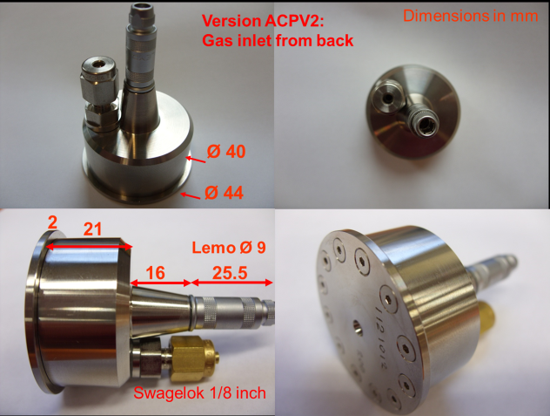
\includegraphics[width=0.75\textwidth]{figures/chap3/piezovalve_picture.png}
	\caption{Labeled picture of the Amsterdam Piezovalve showing dimensions (mm). The gas and electrical connections are located on the rear of the device; the nozzle aperture is located at the center of the front face (flat side).}
	\label{fig:piezovalve_picture}
	% picture supplied by Andrew piper / the manufacturer
\end{figure}

We briefly had access\footnote{Special thanks to fellow graduate student Andrew Piper for letting us borrow his equipment. For more detail and characterization of the piezo valve, see Andrew Piper's dissertation \cite{piperAndrewPiperDissertation2022}.} to a commercial pulsed valve (Amsterdam Piezo Valve by MassSpecpecD BV), as shown in \cref{fig:piezovalve_picture}. The Amsterdam piezo valve utilizes an o-ring mounted to a cantilever piezoelectric flapper to briefly open an internal gas inlet port. This device has a $d = 500 \ \mu \textrm{m}$ diameter straight-channel nozzle and a backing pressure range of 0 - 15 bar. The delay was controlled using a Quantum Composer, the valve opening time was 75 $\mu$s and the operating voltage was 150 V.

The primary motivation for using this device was to complete a two-source harmonic generation experiment (for details, see \cite{hagemanComplexAttosecondTransient2020}), but we performed basic diagnostics on the nozzle after installing it into the TABLe. Recalling \cref{fig:M_rho_vs_x}, the gas density falls off sharply with increasing on-axis distance from the nozzle aperture. However, due to the flat face of the piezo valve assembly, the recessed nozzle aperture and the divergence of the beam, it is difficult to bring the aperture close to the laser axis without obscuring the laser beam and damaging the nozzle. We do not have a direct measurement of the on-axis distance $x$, but we can estimate it using the harmonic yield.

The off-axis density $\rho(x,y,z)$ of a free expansion gas jet is given by \cite{millerFreeJetSources1988}:
\begin{align}
\frac{\rho(x,y,z)}{\rho(x,0,0)} &= \cos^2 \theta \cos^2 \left( \frac{\pi \theta}{2 \phi} \right), \\
\textrm{with} \quad \tan \theta &\equiv \frac{\sqrt{y^2+z^2}}{x},
\label{eqn:off-axis-density}
%note: this eqn is only valid for x > (x/d)_{min}. it isn't valid for HHG experiments.
\end{align}
where $x$ is the on-axis distance from the nozzle aperture, $y$ and $z$ are the off-axis distances from the nozzle's centerline axis (with $z$ parallel to the laser propagation direction), and $\phi$ is a gas constant with values ${\phi = 1.365, 1.662}$, and $1.888$ for ${\gamma = 5/3, 7/5}$ and $9/7$, respectively. If we assume an on-axis gas density distribution $\rho(x,0,0)$ given by \cref{eqn:mach_rho,eqn:Scoles_centerline1} and make the following approximation to \cref{eqn:HHG_Nout} for the harmonic yield $N_{\textrm{out}}$:
\begin{equation}
N_{\textrm{out}}(x, y) \approx \alpha \left| \int_{-\infty}^{\infty} \dd{z} \rho(x,y,z) \right|^2 \textrm{,}
\label{eqn:Nout_approx}
\end{equation}
where $\alpha$ is a scaling constant, then we can extract the on-axis distance $x$ if we measure the harmonic yield as a function of the off-axis distance $y$.

\begin{figure}
	\centering
	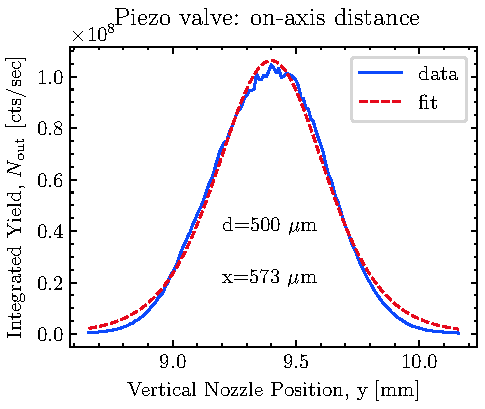
\includegraphics[width=0.75\textwidth]{figures/chap3/piezovalve_vscan.pdf}
	\caption{Integrated yield as a function of off-axis nozzle distance used to determine the on-axis distance, $x$. A fit of \cref{eqn:Nout_approx} to the data yields an on-axis distance of $573 \ \mu \textrm{m}$.}
	\label{fig:piezovalve_vscan}
	% plot made in \Python Scripts\HPC\piezovalve_1450nm.py
\end{figure}

To determine the minimum on-axis distance, we recorded the harmonic yield as a function of the vertical position of the piezo valve relative to a fixed laser focus. This scan was performed using the following optimized generation conditions: a pulse energy of 961 mJ, a fundamental wavelength of 1450 nm at 250 Hz, a CaF\textsubscript{2} generation lens ($f = 40 \ \textrm{cm}$) and 29.3 psig backing pressure of Ar gas. The interaction intensity is estimated to be $3.67 \times 10^{14}$ W/cm\textsuperscript{2}. A 200 $\mu$m metallic aluminum filter located downstream of generation was used to block the fundamental. The experimental data and a fit to \cref{eqn:Nout_approx} are shown in \cref{fig:piezovalve_vscan}. Assuming a nozzle diameter of 500 $\mu$m, we obtain a fit result of $x = 573 \ \mu\textrm{m}$, which represents the closest we can get the laser to the nozzle aperture without damaging the piezo valve assembly. At this distance, the calculated on-axis interaction pressure is 11.7\% of the backing pressure.

\begin{figure}
	\centering
	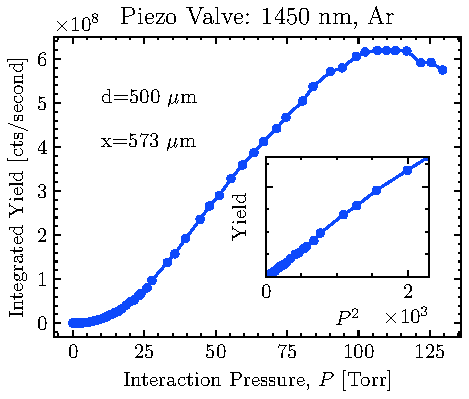
\includegraphics[width=0.75\textwidth]{figures/chap3/piezovalve_pscan.pdf}
	\caption{Integrated harmonic yield from the piezo valve as a function of interaction pressure. The inset shows excellent quadratic behavior with respect to interaction pressure. Assumed on-axis distance is $x = 573 \ \mu \textrm{m}$. To calculate the integrated yield, harmonic spectra are background subtracted, normalized for exposure time and integrated over the sensor area. The total yield has been multiplied by 4 to account for the 250 Hz rep. rate to compare it to the 1 kHz datasets.}
	\label{fig:piezovalve_pscan}
	% plot made in \Python Scripts\HPC\piezovalve_1450nm.py
\end{figure}

\begin{figure}
	\centering
	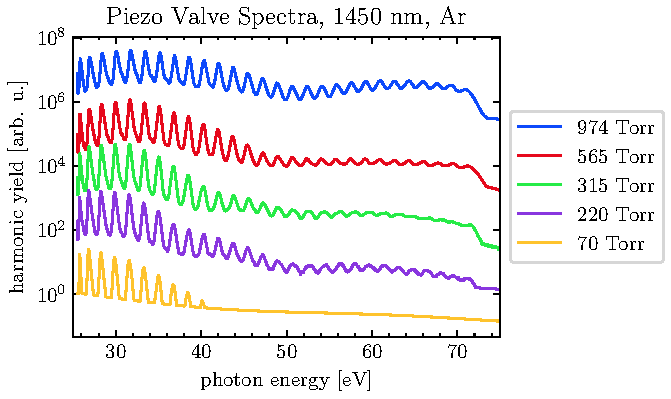
\includegraphics[width=0.9\textwidth]{figures/chap3/piezovalve_spectra.pdf}
	\caption{A selection of piezo valve spectra as a function of interaction pressure. Assumed on-axis distance is $x = 573 \ \mu \textrm{m}$. Normalized yield is calculated by background subtracting the 2D spectra, integrating the spatial dimension of the sensor, normalizing by exposure time and applying the Jacobian. Total yield is multiplied by 4 to account for the 250 Hz laser repetition rate.}
	\label{fig:piezovalve_spectra}
	% plot made in \Python Scripts\HPC\piezovalve_1450nm.py
\end{figure}

As part of a diagnostic process, we recorded harmonic spectra as a function of backing pressure using the aforementioned generation conditions and with the piezo valve centered on the optical axis ($y=0$). The interaction pressure was calculated using \cref{eqn:mach_rho,eqn:Scoles_centerline1} and assuming $x = 573 \ \mu \textrm{m}$, which was unchanged from the previous measurement. The total harmonic yield (below 72.7 eV) is shown in \cref{fig:piezovalve_pscan}. The main figure shows a steadily increasing harmonic yield until a maximum is reached at $\sim 107 \ \textrm{Torr}$, after which the yield starts to decrease. The inset plots the yield as a function of the square of the interaction pressure, which shows excellent quadratic scaling up to 50 Torr.

A select few spectra from this dataset are shown in \cref{fig:piezovalve_spectra}. The sharp decrease in counts at 72.7 eV is due to absorption of the aluminum filter's $L$-edge. As seen in other datasets, the spectral envelope shifts to higher energies with higher pressures, which is consistent with our understanding of the macroscopic phase matching principles discussed in \cref{sec:phase-matching}.

\begin{figure}
	\centering
	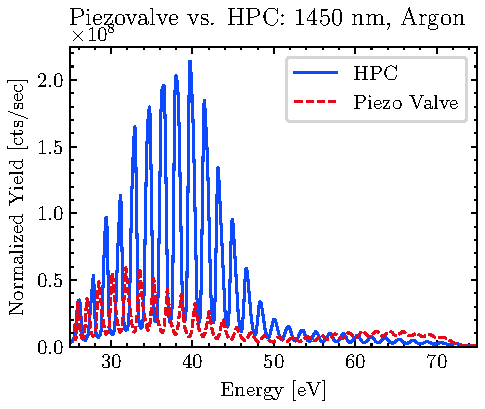
\includegraphics[width=0.75\textwidth]{figures/chap3/HPC_vs_piezovalve.pdf}
	\caption{A comparison of the high pressure cell (HPC) and Amsterdam piezo pulsed valve harmonic yield under typical operating conditions.}
	\label{fig:HPC_vs_piezovalve}
	% plot made in \Python Scripts\HPC\piezovalve_1450nm.py
\end{figure}

\Cref{fig:HPC_vs_piezovalve} compares the performance of the piezo valve compared to the HPC under similar generation and detection conditions. The harmonics were generated using 1450 nm in argon gas, with the spectrometer configured to collect lower energy photons. As before, the spectra have been normalized for exposure time and laser repetition rate. The piezo valve spectra was intentionally blue-shifted for the purposes of an argon spectroscopy experiment \cite{hagemanComplexAttosecondTransient2020}, but this did not affect the overall yield. Note that this data was collected using the full TABLe setup and therefore the absolute XUV yields are not directly comparable to the previous HPC datasets shown in \cref{sec:HPC} due to the additional transmission losses introduced by the ellipsoidal mirror and extra vacuum apertures. Nevertheless, we can see that the HPC's higher interaction pressures and longer effective medium length result in significantly higher yields.

\section{XUV Focal Spot Size}
\label{sec:XUV_knife_edge}

\begin{figure}
	\centering
	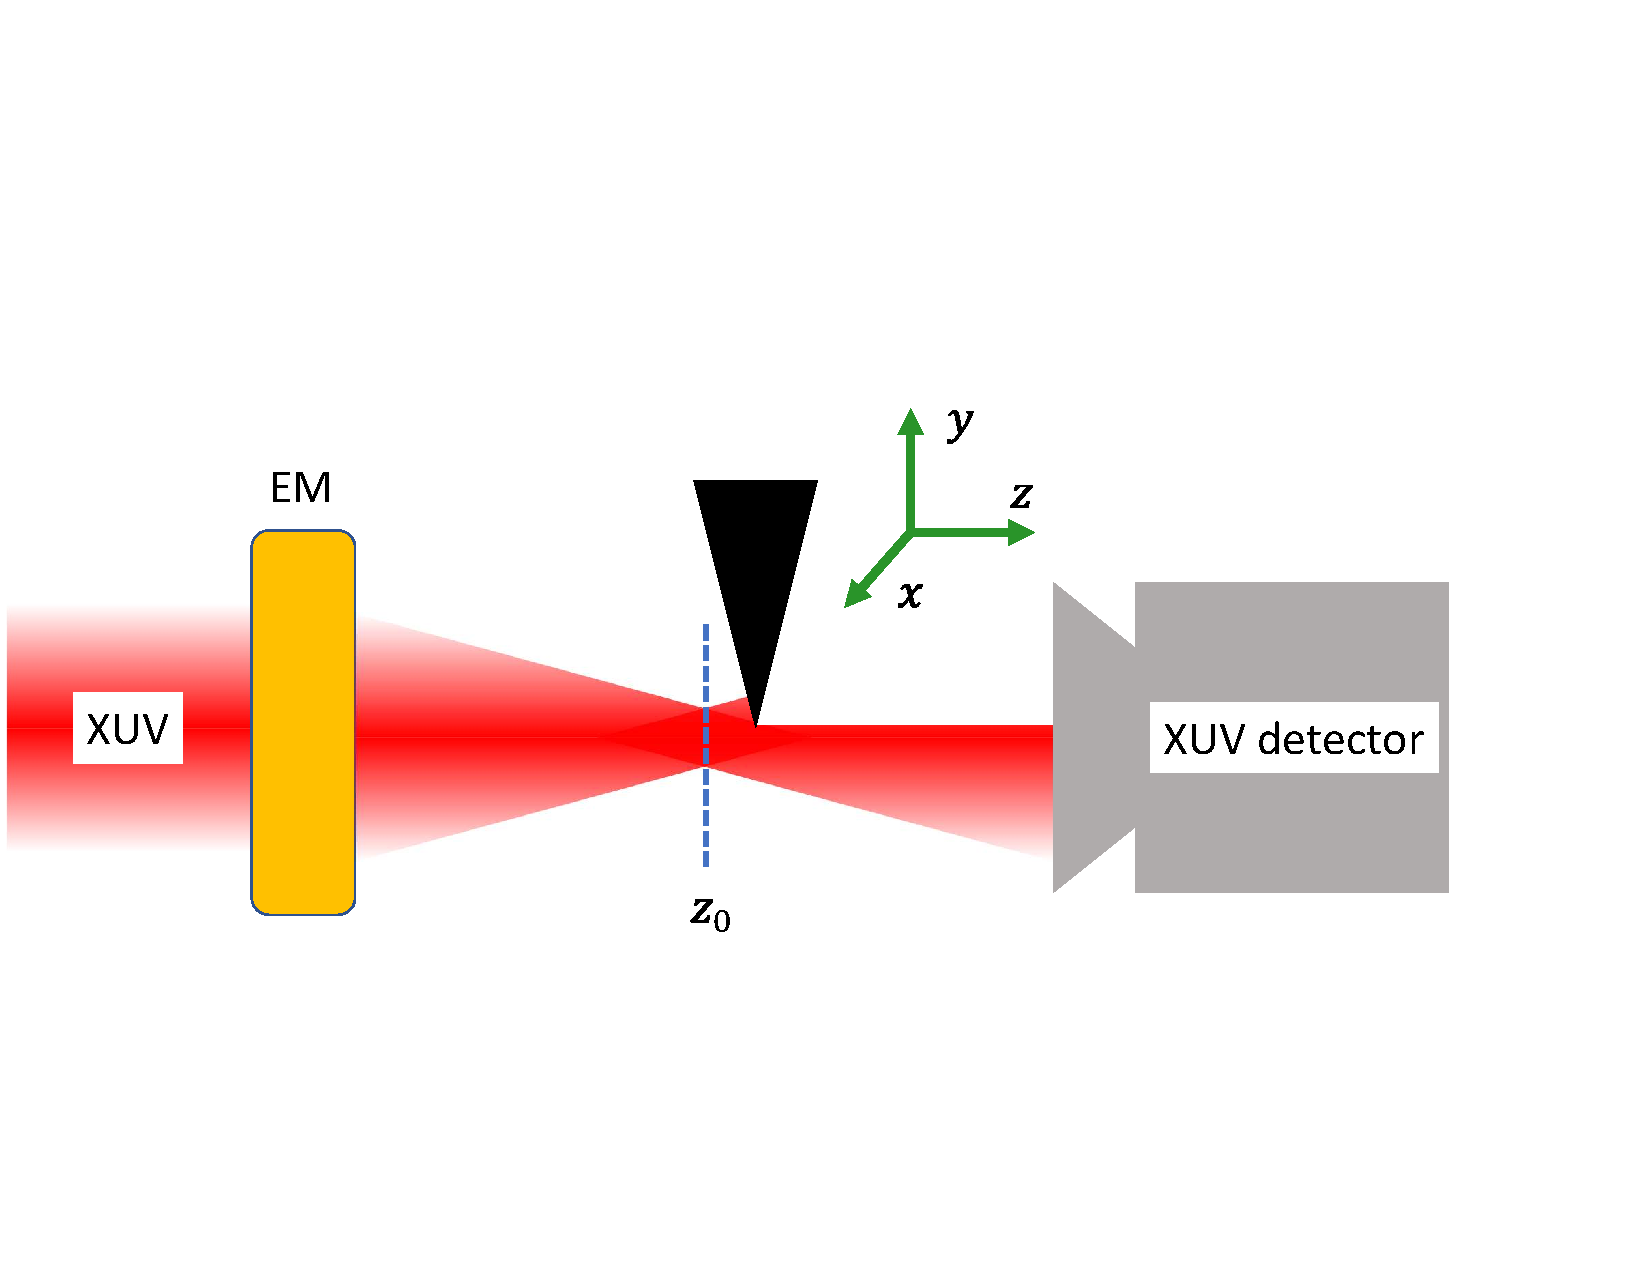
\includegraphics[width=0.9\textwidth]{figures/chap3/knife_edge_cartoon.pdf}
	\caption{Schematic of XUV knife edge measurement. EM: ellipsoidal mirror, $z_0$: XUV focal plane.}
	\label{fig:knife_edge_cartoon}
\end{figure}

A simple knife edge measurement does not give a complete description of the beam profile, but it can be used for basic diagnostic purposes \cite{siegmanHowMaybeMeasure1998,siegmanNewDevelopmentsLaser1990,siegmanDefiningMeasuringOptimizing1993}. The knife edge measurement allows us to locate the extreme ultraviolet (XUV) focus relative to the sample holder, which is critical for pump-probe measurements. Additionally, it can verify the performance of the ellipsoidal mirror and estimate the basic properties of the harmonic generation process.

The edge of a Si frame mounted to the target chamber's sample holder (see \cref{fig:Sample_Geometry}) as our knife edge. The coordinate system geometry is defined in \cref{fig:knife_edge_cartoon}. For this analysis, we assume a Gaussian beam profile with an XUV focus at position $(x_0,y_0,z_0)$ \cite{almeidaHarmonicsBeamsCharacterization2016}:
\begin{equation}
I(x,y,z) = I_0 \left( \frac{w_0}{w(z)} \right)^2 \exp \left[ -2 \frac{ (x-x_0)^2 + (y-y_0)^2 }{w(z)^2} \right],
\end{equation}
The beam waist $w(z)$ will evolve as:
\begin{equation}
w(z) = w_0 \sqrt{ 1 + \left( \frac{z-z_0}{z_R} \right)^2 },
\label{eqn:beam_waist_evolution}
\end{equation}
where $z_R$ is the Rayleigh range. If we use the knife edge to block the transmission as depicted in \cref{fig:knife_edge_cartoon}, then the transmitted power will be:
\begin{equation}
P(y, z) = P_0 + \frac{P_{max}}{2} \left( 1 - \erf \left[ \frac{\sqrt{2}(y-y_0)}{w(z)} \right] \right),
\label{eqn:knife_edge}
\end{equation}
where $y$ is the insertion of the knife in the beam, $z$ represents the location of the knife plane in the propagation direction, and $\erf(\cdots)$ is the error function. To ensure numerical stability during the fitting procedure, we approximate the error function in \cref{eqn:knife_edge} using an analytic function, $f$ \cite{dearaujoMeasurementGaussianLaser2009}:
\begin{equation}
\begin{aligned}
P(y, z) &\approx P_0 + P_{max} f(-s), \\
\textrm{with} \ f(s) &\equiv \frac{1}{1 + \exp(a_1 s + a_3 s^3)}, \\
\textrm{and} \ s &\equiv \frac{2(y-y_0)}{w(z)}, \\
a_1 &= -1.5954086, \\
a_3 &= -7.3638857 \times 10^{-2}.
\end{aligned}
\label{eqn:knife_edge_approx}
\end{equation}

\begin{figure}
	\centering
	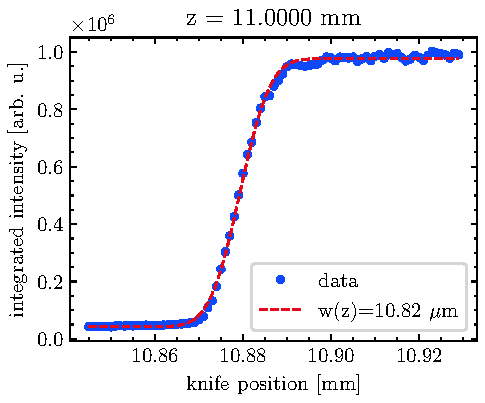
\includegraphics[width=0.75\textwidth]{figures/chap3/XUV_focus_knife_edge.pdf}
	\caption{A typical XUV knife edge measurement near the focal plane. The total harmonic yield was used in this calculation.}
	\label{fig:XUV_focus_knife_edge}
	% dataset: C:\testdata\2019_08_23\knife\11.0000
	% python file: \Python Scripts\Spectrometer\test\knife_edge.py
\end{figure}

\begin{figure}
	\centering
	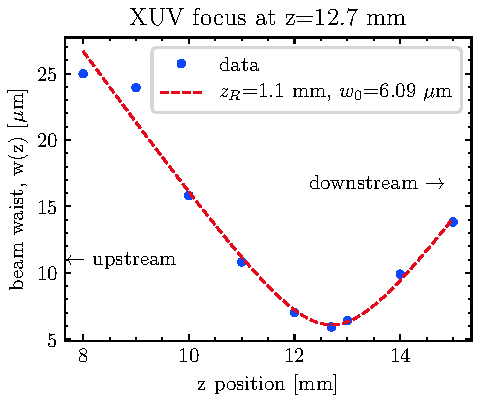
\includegraphics[width=0.75\textwidth]{figures/chap3/XUV_waist_vs_k.pdf}
	\caption{Evolution of XUV beam waist as a function of propagation direction, $z$. The Rayleigh range $z_R$ and beam waist $w_0$ are extracted from the fit to \cref{eqn:beam_waist_evolution}. The total harmonic yield was used in this calculation.}
	\label{fig:XUV_waist_vs_k}
	% question: what is $M^2$ value of the XUV?. or, does w0 and zR change with XUV wavelength?
	% dataset: C:\testdata\2019_08_23\knife\11.0000
	% python file: \Python Scripts\Spectrometer\test\knife_edge.py
\end{figure}

We performed knife edge measurements on harmonics created in argon using a 1430 nm / 715 nm two-color generation scheme (see \cref{sec:HHG_propagation_recombination}). These generation conditions were later used to perform ATAS experiments in germanium. \Cref{fig:XUV_focus_knife_edge} shows the total harmonic signal as the knife edge is inserted into the beam path at a $z$-position near the XUV focal plane. By fitting the data to \cref{eqn:knife_edge_approx}, we obtain the local waist radius $w(z)$. This measurement is repeated for different $z$ values until the focal plane is found, as shown in \cref{fig:XUV_waist_vs_k}. The Rayleigh range $z_R$ and focal spot size $w_0$ are found by fitting the evolving beam waist data to \cref{eqn:beam_waist_evolution}.

\begin{figure}
	\centering
	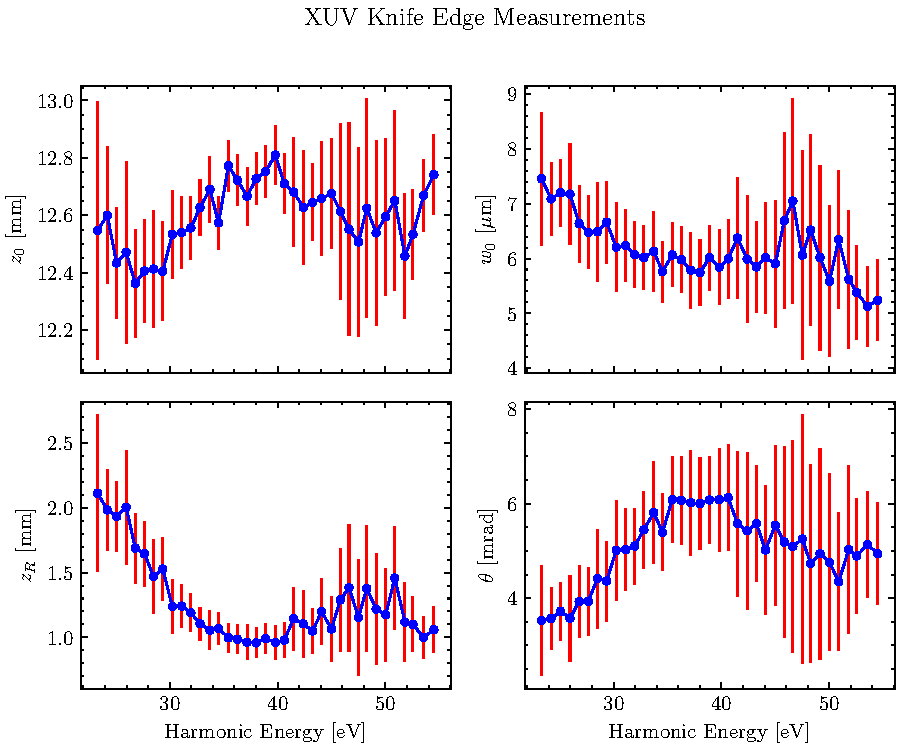
\includegraphics[width=1.0\textwidth]{figures/chap3/knife_edge_fit_2x2.pdf}
	\caption{Energy-resolved fit parameters following a knife edge measurement of two-color harmonic spectrum generated in argon using 1430 nm / 715 nm light. The focal plane position ($z_0$), beam waist radius ($w_0$), Rayleigh range ($z_R$), and half-angle divergence ($\theta$) are calculated for each harmonic. Error bars represent one standard deviation on the parameters.}
	\label{fig:knife_edge_fit_2x2}
	% python file: \Python Scripts\Spectrometer\test\knife_edge.py
\end{figure}

This calculation was performed for each harmonic in the spectrum. \Cref{fig:knife_edge_fit_2x2} shows the energy-resolved parameters for 37 harmonics ranging from $\sim 23.4 \ \textrm{eV}$ to $\sim 54.5 \ \textrm{eV}$. The far-field divergence half-angle $\theta$ is calculated from the fit parameters in \cref{eqn:beam_waist_evolution} via $\theta = \arctan(w_0 / z_R)$. Neglecting geometric losses from the finite aperture of the ellipsoidal mirror, we estimate the divergence of the harmonics after generation to be $M = 3$ times smaller than at the XUV focus. This gives us a harmonic divergence immediately after generation ranging from $\theta \simeq 1.1 - 2 \ \textrm{mrad}$, which is consistent with what is reported in the literature \cite{tischAngularlyResolvedHighorder1994}.

We don't know the size of the XUV generating volume in the generation chamber, so we can't use the measured spot size to comment on the performance of the ellipsoidal mirror. However, we note that this XUV spot size is what we expect given our generation conditions. For a focal length of $f = 40 \ \textrm{cm}$ and an input beam diameter of $D = 10 \ \textrm{mm}$, the 1430 nm light will have a beam waist radius $w_0 = (2 \lambda / \pi)(f/d) = 36.4 \ \mu \textrm{m}$, and the 715 nm light will have $w_0 = 18.2 \mu \ \textrm{m}$. With a demagnification factor of $M=3$, an XUV beam waist radius of 6 $\mu$m in the target chamber corresponds to an 18 $\mu$m beam waist in the generation chamber. This means that the XUV light is generated in a volume approximately half the size of the fundamental beam's spot size.

\section{Microchannel Plate (MCP) response}
% MCP voltage data taken on 2019_10_07.

\begin{figure}
	\centering
	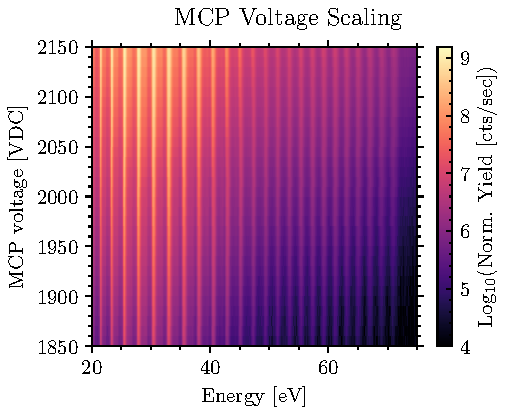
\includegraphics[width=0.75\textwidth]{figures/chap3/MCP_voltage_spectro.pdf}
	\caption{Harmonic spectra as a function of MCP voltage. Harmonics were generated in argon gas with a 1250 nm fundamental. The aluminum $L$-edge is visible at 72.7 eV.}
	\label{fig:MCP_voltage_spectro}
	% python file: \Python Scripts\Spectrometer\test\MCP_gain_voltage.py
\end{figure}

\begin{figure}
	\centering
	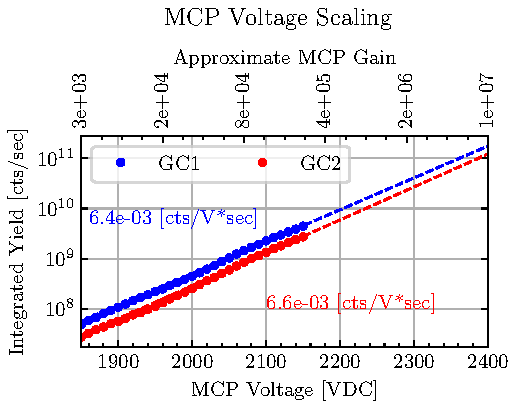
\includegraphics[width=0.9\textwidth]{figures/chap3/MCP_voltage_sum.pdf}
	\caption{Integrated harmonic yield $Y$ as a function of MCP voltage. GC1 was obtained by summing the spectra in \cref{fig:MCP_voltage_spectro}, GC2 was taken under similar but slightly less efficient harmonic generation conditions. Approximate gain is calculated assuming $G = 10^7$ at 2400 VDC and using the fitting coefficient from GC1.}
	\label{fig:MCP_voltage_sumo}
	% python file: \Python Scripts\Spectrometer\test\MCP_gain_voltage.py
\end{figure}

The gain of the MCP can be controlled by adjusting the accelerating voltage between the microchannel plates. This scaling is demonstrated experimentally in \cref{fig:MCP_voltage_spectro,fig:MCP_voltage_sumo} using harmonics generated in argon gas with a 1250 nm fundamental. Near typical operating voltages, the measured harmonic yield $Y$ follows a power law of the form \cite{fraserGrayImagingUsing1984,ladislaswizaMicrochannelPlateDetectors1979a}:
\begin{equation}
Y = b * 10^{m V},
\label{eqn:MCP_gain_function}
\end{equation}
where $b$ and $m$ are fitting coefficients, and $V$ is the operating voltage of the MCP array in Volts.

In \cref{fig:MCP_voltage_spectro}, we see that the MCP signal increase is spatially uniform across the sensor. \Cref{eqn:MCP_gain_function} shows the integrated yield for two generating conditions (GC1 and GC2) and a fit to \cref{eqn:MCP_gain_function}. The slopes $m$ are noted in the figure. We see that an increase of 100 V increases the measured signal by a factor of $\sim 4.5$.

According to the manufacturer, typical gain values are at least $10^7$ at 2400 VDC. As we do not have access to a known-brightness XUV source, we are unable to measure the gain directly. We estimate the MCP's gain $G$ by assuming $G = 10^7$ at 2400 VDC and scaling it using the fitting coefficients obtained from the GC1 dataset. Using this assumption, we estimate $G(\textrm{2000 VDC}) \approx 3 \times 10^4$, and $G(\textrm{2150 VDC}) \approx 3 \times 10^5$.

According to the manufacturer, dielectric breakdown may occur when the voltage across the plates is in excess of 2400 VDC. Additionally, the plates are consumable, as they only support a finite amount of charge transfer before needing replacement. In the interest of extending the lifetime of the equipment, it is good practice to optimize experimental conditions at a relatively low voltage (2000 VDC) and only increase the voltage to higher values when collecting data for sensitive experiments. For this reason, most experiments are performed with the plate voltage below 2200 VDC.


\section{Conclusion}

We have developed a new gas source for high harmonic generation (the HPC) and modeled the gas flow within it. The measured vacuum performance was shown to agree with this model, which was then used to calculate the interaction pressure during the high harmonic generation process. The high harmonic yield of the HPC was measured under a variety of generating conditions, and it compared favorably to the other HHG gas sources available in the lab. When generating in helium at 800 nm, the XUV flux of the high pressure cell is up to 150 times brighter than the LPC, and 4 times brighter than the piezo valve when generating in argon at 1450 nm. Although we don't have direct measurements for comparison, we estimated the HPC would be between 1 and 2 orders of magnitude brighter than the LPC when operated at 1450 nm using argon. Since the optimal interaction pressure  $P_{\textrm{opt}}$ scales with $\lambda^2$, we expect the HPC to become more relevant at longer wavelengths, for example when using the lab's fiber compressor to achieve few-cycle pulses at ${\lambda = 1.8 \ \mu \textrm{m}}$ \cite{gormanAttosecondProbingElectron2018}. The performance of the XUV focusing element was also validated using a knife edge measurement at the sample focus, and we characterized the divergence of the beam across its bandwidth. Finally, we validated the performance of the microchannel plate (MCP) and we estimated its gain over a range of operating voltages. In the next chapter, we use the increased harmonic flux to perform transient absorption measurements in germanium.
